%%%%%%%%%%%%%%%%%%%%%%%%%%%%%%%
%%  INTRO AND MOTIVATION 
%%%%%%%%%%%%%%%%%%%%%%%%%%%%%%%

\chapter{The Earth-Sun System}\label{ch:earth_sun} 
\chapterauthor{Colin Adams\footnote{Colin Adams completed all the research, writing, and developed the graphics for this chapter.}}

\section{\label{sec:pbd}The Pale Blue Dot}

\subsection{Voyager 1's Legacy}

On September 5, 1977, the \emph{Voyager 1} space probe was launched into space by the United States' National Aeronautics and Space Administration (NASA). The space probe's mission was to explore the outer solar system, specifically, to study Jupiter and Saturn. In 1990, after completing its original purpose,  \emph{Voyager 1} received a new mission: take a solar system ``family portrait.'' That is, from a distance of approximately 6 billion kilometers from the sun, \emph{Voyager 1} would take pictures of six planets and their relative positions by combining different images together.

On February 14, 1990  \emph{Voyager 1} turned around and pointed its camera back at Earth. It took 60 different photos of the solar system (see Figure~\ref{fig:EarthSunVenus}) and sent them back to Earth where they were stitched together. It took over five and a half hours to transmit the photographic data across the vast expanse of space, from \emph{Voyager 1} back to Earth. 

    \begin{figure}[ht]
    \centering
		\includegraphics[width=0.55\textwidth]{SunEarthVenus_PBD.png}
		\caption{A picture of the sun and inner solar system. Superimposed on the left side are pictures of Venus and Earth (see Figure~\ref{fig:pale_blue_dot}). This is what \emph{Voyager 1} saw nearly 6 billion \si{\km} away from the sun. Image taken from NASA/JPL.}
        \label{fig:EarthSunVenus}
    \end{figure}

Three of the sixty photographs contained Earth as a single point of light. By processing these three photographs, NASA was able to produce an image of the earth taken over six billion kilometers away from the sun. In each case, Earth was less than a single pixel in each of the photographs %\citep{planetary}.

    \begin{figure}[ht]
    \centering
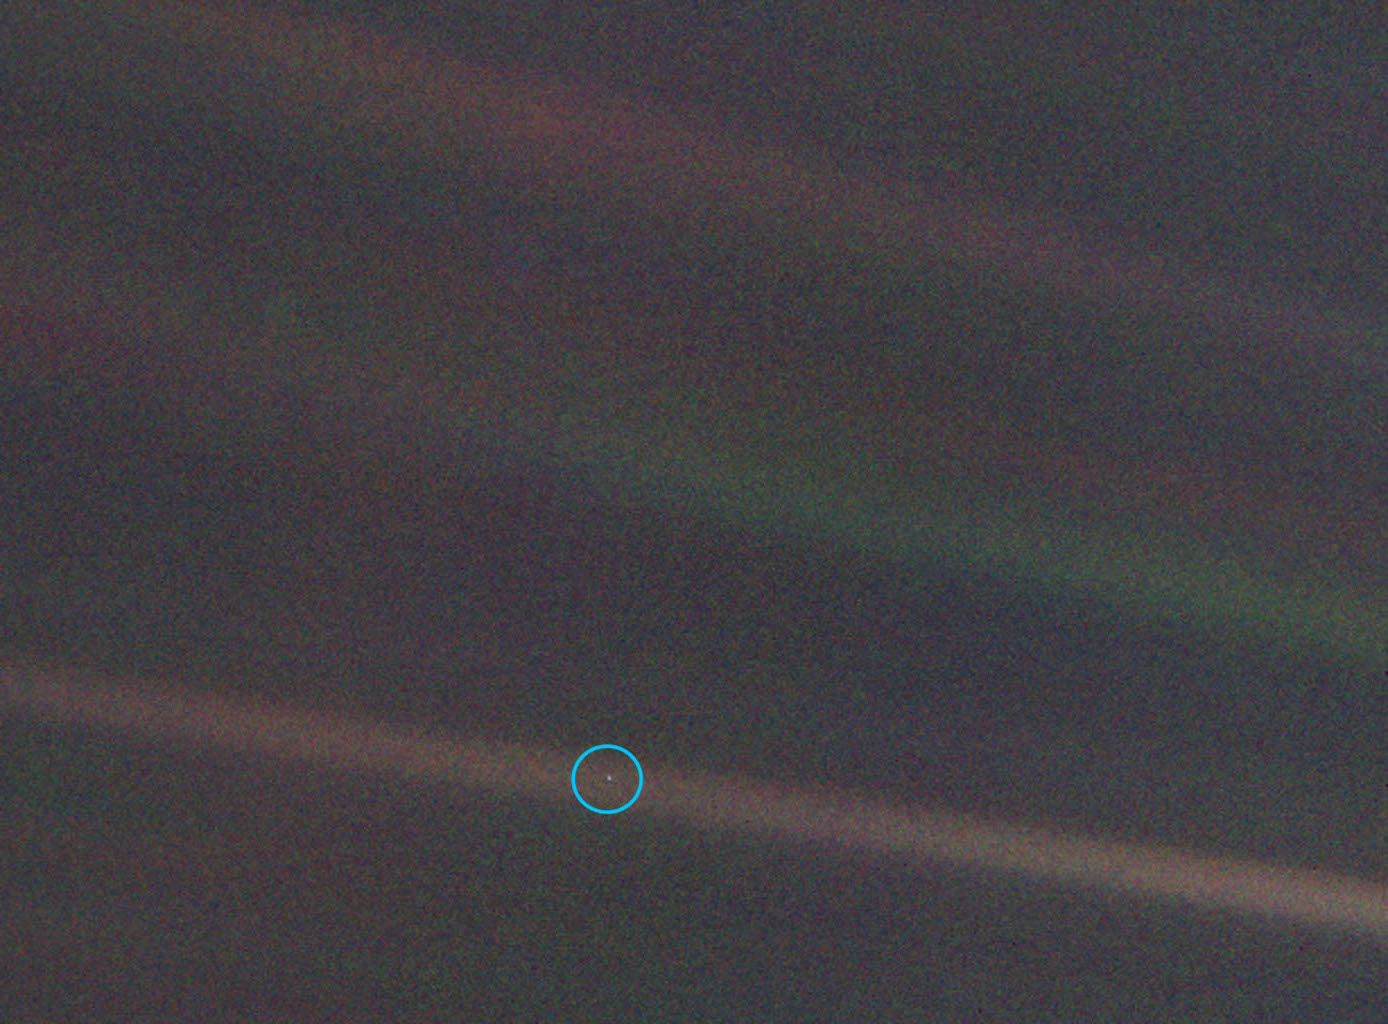
\includegraphics[width=0.70\textwidth]{PaleBlueDot.jpg}

        \caption{The Pale Blue Dot. This is perhaps the most famous photograph taken by \emph{Voyager 1} on February 14, 1990. The the size of the Earth is less than a single pixel. The Earth is circled for clarity. Image taken and modified from NASA/JPL.}
        \label{fig:pale_blue_dot}
    \end{figure}

    Coincidentally, when the photograph was taken, sunlight scattered across the lens of the camera, creating the illusion that the earth was caught in a ray of light from the sun (see  Figure~\ref{fig:pale_blue_dot}). In his book, astronomer Carl Sagan commented upon this image and its significance:
    \begin{displayquote}
        \small %change font size to distinguish quote from rest of text
        \quad Look again at that dot. That's here. That's home. That's us. On it everyone you love, everyone you know, everyone you ever heard of, every human being who ever was, lived out their lives. The aggregate of our joy and suffering, thousands of confident religions, ideologies, and economic doctrines, every hunter and forager, every hero and coward, every creator and destroyer of civilization, every king and peasant, every young couple in love, every mother and father, hopeful child, inventor and explorer, every teacher of morals, every corrupt politician, every ``superstar,'' every ``supreme leader," every saint and sinner in the history of our species lived there---on a mote of dust suspended in a sunbeam.

        \quad The Earth is a very small stage in a vast cosmic arena. Think of the rivers of blood spilled by all those generals and emperors so that, in glory and triumph, they could become the momentary masters of a fraction of a dot. Think of the endless cruelties visited by the inhabitants of one corner of this pixel on the scarcely distinguishable inhabitants of some other corner, how frequent their misunderstandings, how eager they are to kill one another, how fervent their hatreds.

        \quad Our posturings, our imagined self-importance, the delusion that we have some privileged position in the Universe, are challenged by this point of pale light. Our planet is a lonely speck in the great enveloping cosmic dark. In our obscurity, in all this vastness, there is no hint that help will come from elsewhere to save us from ourselves.

        \quad The Earth is the only world known so far to harbor life. There is nowhere else, at least in the near future, to which our species could migrate. Visit, yes. Settle, not yet. Like it or not, for the moment the Earth is where we make our stand.

        \quad It has been said that astronomy is a humbling and character-building experience. There is perhaps no better demonstration of the folly of human conceits than this distant image of our tiny world. To me, it underscores our responsibility to deal more kindly with one another, and to preserve and cherish the pale blue dot, the only home we've ever known \cite{sagan}.
    \end{displayquote}

    With this perspective, we delve into the study of the earth, its environment, and us. We attempt to unearth our interactions with and our impacts on our only home. To begin, we look at the interaction between the earth and its main source of energy: the sun. By doing this, we will understand the greenhouse effect and its necessity by looking at very crude models of the earth and its atmosphere. 

    %%%%%%%%%%%%%%%%%%%%%%%
    %% FORMATION OF SS
    %%%%%%%%%%%%%%%%%%%%%%%

    \section{\label{sec:solar_sys}Formation of the Solar System}
		
		\subsection{The Nebular Hypothesis}

    Nobody is entirely sure how the solar system formed, but there are a few \textbf{hypotheses} on how it did. Here, we will present the Nebular hypothesis of its formation.

    As we know it today, the solar system is anywhere from 4.5 to 4.8 billion years old. Scientists believe stars form from huge clouds of gas (called a \textbf{nebulae}) and other, heavier elements. The gas is compressed by gravity, becoming more and more dense until the gas gets so hot that two protons combine to form helium. %\footnote{
        % This is not the complete picture. If p is a proton, d is deuterium (a proton and neutron binded together), e$^+$ is a positron (anti-electron), $\nu_e$ is a neutrino, and $\gamma$ is a high energy photon, then the actual reaction looks something like:
        % \begin{align*}
        % \text{p} + \text{p} &\to \text{d} + \text{e}^{+} + \nu_e + \SI{0.4}{\mega \electronvolt}\\
        %   \text{d} + \text{p} &\to {}^3\text{He} + \gamma + \SI{5.5 }{\mega \electronvolt} \\
        %   {}^{3}\text{He} + {}^3\text{He} &\to {}^4\text{He} + \text{p} + \text{p} +  \SI{12.9}{\mega \electronvolt}
        % \end{align*}
        % If we add two of the first and second reaction to one of the third reaction we get the overall reaction of
        %     \[
        %     4 \text{p} \to {}^4\text{He} + 2\text{e}^{+} + 2\nu_e + \SI{24.7}{\mega \electronvolt}
        %     \]
        % which effectively turns hydrogen into helium; N.B.: \SI{1}{\electronvolt} = \SI{1.602e-19 }{\joule}. This is not crucial for developing a good understanding and can be skipped, however I leave it here for the interested reader \citep{thorndike1976energy,townsend2010baby}}
    This process is known as \textbf{nuclear fusion}. When fusion occurs, the star releases a tremendous amount of energy in the form of electromagnetic radiation---such as visible light, infrared light (IR), x-rays, ultraviolet (UV) rays, radio waves, etc.---and the ball of gas begins to shine. When this happens, a star is born. Like every star, the sun was formed after the gravitational collapse of a nebula. This process occurred over the course of about a million years \citep{formation_solar}.

    In the process of this formation, a disk of gas and other elements caught by the sun's immense gravitational pull began to clump together to form grains that collided into one another, becoming bigger, and bigger. Over the course of 10--100 million years, these grains collided and merged until they became large enough to form the planets of our solar system \citep{hayashi1985formation}.

\subsection{Rocky versus Giant Gas Planets}

    The \textbf{terrestrial planets}, also known as the rocky planets, (e.g. Mercury, Venus, Earth, and Mars) are closest to the sun because the inner solar system was too warm to for volatile molecules to be structurally important for the planet. Thus, only elements with higher melting points (iron, nickel, silicon, etc.) could remain in this region. When the planets got large enough, the terrestrial planets' gravity was strong enough to maintain an atmosphere. Unsurprisingly, the more massive a planet is (i.e. the stronger its gravity) the more equipped it is at maintaining its atmosphere. For example, studies have shown that Mars had a much thicker atmosphere with a different composition in the past than it does today, more similar to Earth's. However, Mars has about $1/10$ the mass that Earth does. Current hypotheses believe that solar wind destroyed much of Mars' atmosphere, as it's gravitational field was unable to maintain it while Earth's remained intact despite being closer to the sun \citep{owen1992composition}. Much of the remaining gas of the nebula formed into the much larger \textbf{gas giants} in the outer solar system (Jupiter, Saturn, Uranus, and Neptune) or was blown away by solar wind \citep{hayashi1985formation}.

    Over the next few billion years, the solar system evolved into what we see today. At some point along the way, water formed on the surface of the earth and life soon followed---exactly how remains one of the great mysteries of modern science. Over billions of years, life evolved into what we see around us today \citep{bell2015potentially} As life enveloped the earth's surface, spreading to every corner, it changed everything from its the physical surface to the composition of the atmosphere.

    %%%%%%%%%%%%%%%%%%%%%%%%%%%%%%%%%%%
    %%   ENERGY TRANSFER B/W E+S
    %%%%%%%%%%%%%%%%%%%%%%%%%%%%%%%%%%%

    \section{\label{sec:energy_flow}Global Energy Flow}
		
\subsection{Radiant Energy Impinges on the Earth's Atmosphere}

    The earth's principal source of energy comes from the sun which releases radiant energy that impinges upon the earth's atmosphere.  Some of this energy is reflected back into space by clouds, some is absorbed by the clouds themselves, while some penetrates through the atmosphere making it to the earth's surface, where it is again either reflected or absorbed. Some of the energy is indeed reflected (water, snow, ice, clouds---in what is known as the \textbf{albedo effect}). Once it makes it to the earth's surface, it is absorbed and \emph{re-radiated}.

    When this energy is absorbed by the surface, it warms the soil or water. The warmer soil and water can transfer energy from the surface to the lower atmosphere by \textbf{conduction}. The warmer, lower atmosphere transfers energy horizontally and vertically of the upper atmosphere layers through \textbf{convection}.\footnote{
        Conduction is the direct transfer of heat or electricity without the movement of the material. Convection is the transfer of heat through the movement caused within a fluid. A good example to keep the two straight in your head would be a wood-fired furnace. When you touch the furnace (and probably burn your hand), you are warming your hand through direction contact with a material, i.e. conduction. When you place your hand just above the furnace (the safer thing to do), you are letting the air (a fluid) warm your hand through by first warming the surrounding air that is transfered to your hand, i.e. convection.
        } 
				
    In addition to all of this, the atmosphere can lose some of this heat by re-radiating some of this energy in the form of infrared light. This infrared light can either be sent back to the earth's surface, ejected into space, or re-absorbed somewhere else in the atmosphere. Eventually, the vast majority of the energy that has entered near the earth will leave it. 

    If this process seems like a complicated, then you are correct! What was described above is what ultimately determines the earth's temperature, climate, and weather.
		
\subsection{Energy is Conserved}

    Because energy is always conserved and there is negligible energy that is gained by the earth, there is a balance between the amount of energy the earth receives from the sun and the amount it radiates away over a given period of time. In other words, the earth and the sun are in \textbf{equilibrium} with each other \citep{thorndike1976energy}. If they were not, the earth would continue to get warmer and warmer over time until it was in equilibrium with the sun. However, when considering the whole surface of the earth, the surface temperature is essentially constant implying an equilibrium. To emphasize this point once more, the earth radiates away energy at the same rate it receives it from the sun. This will be the fundamental basis for the rest of the chapter where we will use very simple models in order to gain a better understanding of the earth, its atmosphere, and the greenhouse effect.


        \subsection{The Sun and the Solar Constant} % (fold)
        \label{sub:the_sun}
        
        The sun is approximately \SI{1.5e8}{\km} away from the earth with a surface temperature of about \SI{5800}{\kelvin}. By simply knowing the temperature of the sun's surface as well as its distance away from the earth, we are able to calculate the frequency distribution of the light emitted by the sun (Figure~\ref{fig:sun_bb}) as well as its brightness. This is because, to a very good approximation, the sun (and the earth, as we will later see) behaves as a blackbody which emits \textbf{blackbody radiation}. You probably are familiar with the idea of blackbody radiation whether you know it or not. When an object is at a certain temperature, it emits light centered around a peak wavelength and other wavelengths of light are distributed about this peak. The distributions of emitted light from objects at different temperatures have similar shapes but have their peak wavelength value at a different value. The hotter the object, the shorter its wavelength and the bluer it looks. This is why hot objects glow red, hotter objects glow blue, and even hotter objects glow white. We can treat both the sun and the earth as objects at a certain temperature. The sun mostly emits visible light while the earth emits infrared light (See Figure~\ref{fig:sun_bb} and Figure~\ref{fig:earth_bb} for a visual representation of this).

        The surface temperature of the sun as well as its distance from Earth is enough information to calculate a value called the \textbf{solar constant}, which we will denote by $\mathcal{S}$ in this text. The solar constant tells us the amount of solar energy per unit time and per unit area the earth receives. The units are \si{\joule/\second/\meter^{2}} = \si{\watt/\meter^{2}}. A joule, denoted by \si{\joule}, is a unit of energy. For a concrete example, an object that has a mass of \SI{2}{\kg} that is moving at \SI{1}{\m/\s} has one joule of energy. The amount of energy released during a given period of time is a measure of power. Here we use watts as the unit of power, which is denoted by \si{\watt}, and is defined to be $\SI{1}{\watt} = \SI{1}{\joule/\s}$. 

        One way to visualize what the solar constant actually means is to imagine a unit of area (in this case, one square meter) that is placed just above the earth's atmosphere oriented such that the sun shines squarely on it. The amount of energy (measured in joules) that flows through that area in a given amount of time (in this case, one second). This solar constant has been measured to be $\mathcal{S} = \SI{1370}{\watt/\m^2}$ \citep{schroeder1999introduction,thorndike1976energy}p
        % subsubsection the_sun (end)

        \begin{figure}[ht]
            \centering
            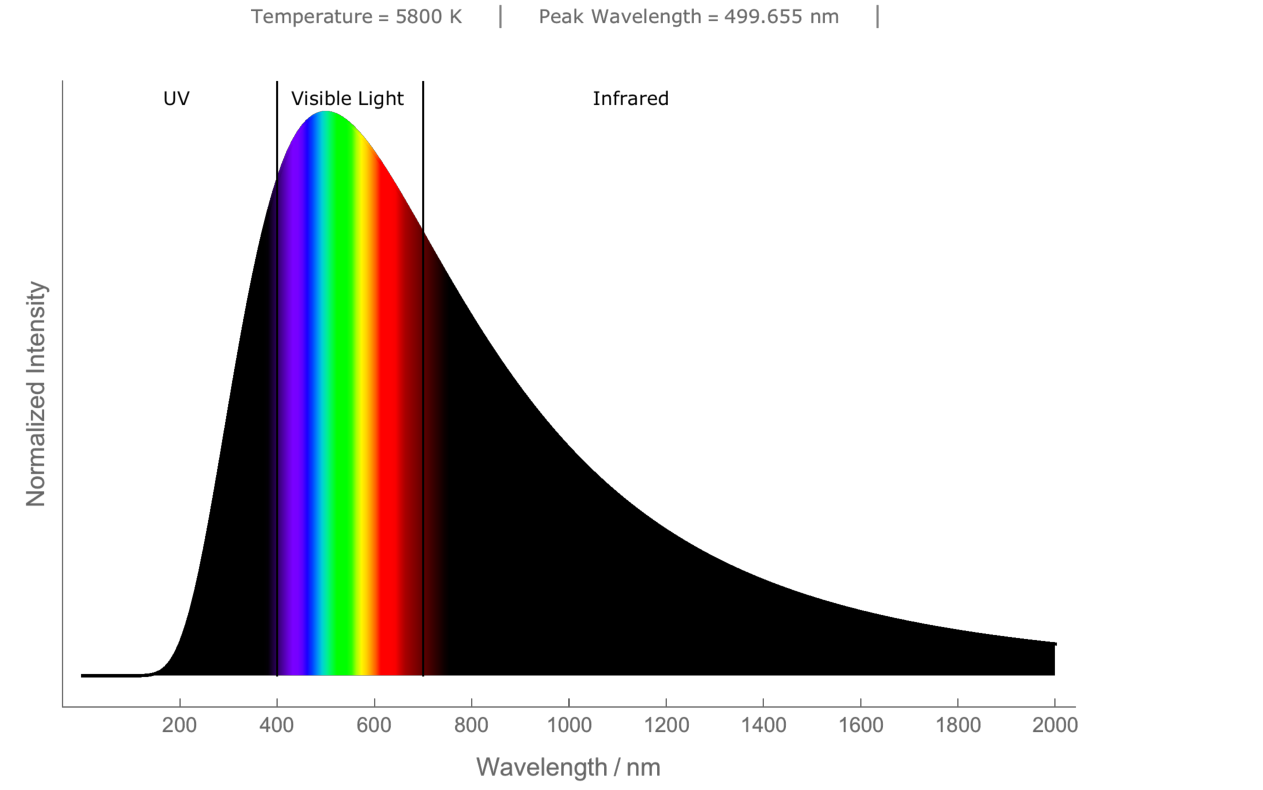
\includegraphics[width = 0.8\textwidth]{sun_blackbody.pdf}
            \caption{The intensity of light as a function of wavelength for an object the same temperature as our Sun (\SI{5800}{\kelvin}). This distribution of wavelengths is only dependent on the temperature of the object. The black portions of the distribution are wavelengths of light that human eyes cannot detect. Looking at this, you should realize that it is no coincidence that life on Earth managed to evolve to see in the visible spectrum of light.}
            \label{fig:sun_bb}
        \end{figure}

        We have already discussed that the earth and the sun are in equilibrium with one another. Again, this simply means that the earth is radiating the same amount of energy into space as it receives from the sun in a given period of time. The total power (energy per unit time) that is emitted by an object is given by
        \begin{equation}
            \text{power} = \sigma e A T^4
            \label{eq:stefan_law}
        \end{equation}
        where $T$ is the object's temperature, $A$ is the object's area, $e$ is the object's emissivity,\footnote
        {
            The emissivity is the fraction of light absorbed at a particular wavelength. For an object that absorbs all incoming light (a blackbody) then $e = 1$; an object that reflects all light would have $e = 0$.
        } 
        and $\sigma$ is the Stefan-Boltzmann constant\footnote
        {
            This is just a constant (with units!), and is rather easy to remember. Just think ``5-6-7-8'' but don't forget the minus sign in front of the 8.
        } 
        where 
        \begin{equation}
            \sigma = \SI[per-mode=fraction]{5.67e-8}{\watt \per (\meter^2  \kelvin^4)}. 
        \end{equation}
        Equation~(\ref{eq:stefan_law}) is known as \textbf{Stefan's Law}. An important point: when using Eq.~(\ref{eq:stefan_law}), you must be careful to use the correct temperature units of Kelvin. To convert between Celsius and Kelvin we have a conversion formula of $T_K = T_C + 273.15$ where $T_K$ is the temperature in Kelvin and $T_C$ is the temperature in Celsius.

        \begin{exercise}
            What is the temperatures of water's
            \begin{enumerate*}[(a)]
                \item  freezing point (\SI{0}{\celsius})
                \item and boiling point at sea level (\SI{100}{\celsius})
                given in kelvin?
            \end{enumerate*}
        \label{ex:kelvin}
        \end{exercise}

        \begin{exercise}
        If a person's body has a surface area of roughly \SI{1.4}{\meter^2} and a  temperature of \SI{37}{\celsius} (take $e = 1$):
            \begin{enumerate}[(a)]
                \item How much power does a person give off? 
                \item Compare the total \underline{energy} radiated by your body in one day compared to the energy in the food that you eat. Why is there such a large discrepancy? (Note that $\SI{1}{\text{Calorie}}=\SI{4184}{\joule}$).
            \end{enumerate}
            \label{ex:humans}
        \end{exercise}

    \subsection{The Dark Earth Model} % (fold)
    \label{sub:dark_earth}

    Now we are finally able to model the energy flow to and from the earth. However, the ``earth'' that we will first be describing will be a rather simple one: it will have no atmosphere and no oceans. We will also assume that this earth is a perfect blackbody (with $e =1$), meaning that it reflects \emph{no} incident radiation from the sun. Previously, we argued that earth was in equilibrium with the sun. Again, the rate at which the earth receives energy from the sun is the same as the rate the earth expels energy. So if we balance the amount of energy flowing from the sun to the earth over a given period of time, ($\mathcal{S}$), and set it equal to the amount of energy being emitted by the earth over a given period of time, we can calculate the surface temperature of the earth. That is, we have
    \begin{align}
        \mathcal{S}\underbrace{(\pi R^2)}_{A_{circ}} = \underbrace{(4\pi R^2)}_{A_{sph}} \sigma T^4
        \label{eq:earth_balance}
    \end{align}
    where $R$ is the radius of the earth and $T$ is the surface temperature of the earth. Now each term contained within parentheses of Eq.~(\ref{eq:earth_balance}) is the relevant area. On the left-hand side of the equation, the sun only sees the earth as a circular disk, hence we use the area of a circle $A_{circ} = \pi r^2$. However, the earth emits this radiation from all directions of a sphere, which---you may remember from geometry---has a surface area of $A_{sph} = 4 \pi r^2$. When we solve for the temperature, $T$, in Eq.~(\ref{eq:earth_balance}) we get 
    \begin{align}
        T = \left( \frac{\mathcal{S}}{4 \sigma} \right)^{1/4} = \left( \frac{\SI{1370}{\watt/\meter^2}}{4 \cdot \SI{5.67e-8}{\watt/(\meter^2 \kelvin^4)} } \right)^{1/4} = \SI{279}{\kelvin}
        \label{eq:earth_temp}
    \end{align}
    which is actually a really good estimate for the earth's equilibrium temperature because the average surface temperature is measured to be \SI{288}{\kelvin} (\SI{15}{\celsius}) \citep{schroeder1999introduction} In fact, this simple model agrees too well! We had no right to be this close to what we measure with the crudeness of our assumptions. This will become apparent when we refine the model in Sec.~\ref{sub:shiny_earth}. However, before moving on to a better model, we should discuss the stability of the earth-sun system by discussing the concept of \textbf{feedback}---a process in which a system reacts to an action or behavior.


    \subsubsection{Feedback---A Digression} % (fold)
		
		\textcolor{red}{[LET'S MAKE THIS INTO A TEXT BOX -- PROBABLY USING MINIPAGE FUNCTIONS.]}
    \label{ssub:feedback}
    Feedback loops crop up all over the natural world and are especially prominent when studying the environment. Because of this, being able to recognize and identify various feedback loops is an important skill to have.
    
    Consider three balls placed on three different surfaces: one on a concave surface, one on a flat surface, and one on a convex surface as illustrated in Figure~\ref{fig:feedback}. When placed on the surfaces at rest and left undisturbed, the three balls will remain at rest forever; however, if the balls are slightly bumped then there are three very different responses. 

    The concave ball (the leftmost) will try to return back to its starting location if displaced. This is known as a \textbf{stable equilibrium}. The initial displacement leads the ball to feel a restoring force pushing it back to where it started. The restoring force in this case would be gravity, and it is said to provide \textbf{negative feedback}. For the ball in the center, we have a situation of \textbf{neutral equilibrium}. If displaced it, it will simply have changed locations but will not return or roll away from its original position. There is \textbf{no feedback} in this situation. Lastly, for a ball on a convex surface (an \textbf{unstable equilibrium}), if it is nudged slightly, the ball will experience a force forcing it away from its equilibrium. As you may have guessed, this is an example of \textbf{positive feedback}. The adjectives of ``positive'' and ``negative'' are not meant to convey ``good'' or ``bad,'' rather they express the direction the system will move towards after being displaced: ``positive'' means move away from where it started whereas ``negative'' means returning to where it started.

    \begin{figure}[ht]
    \centering
    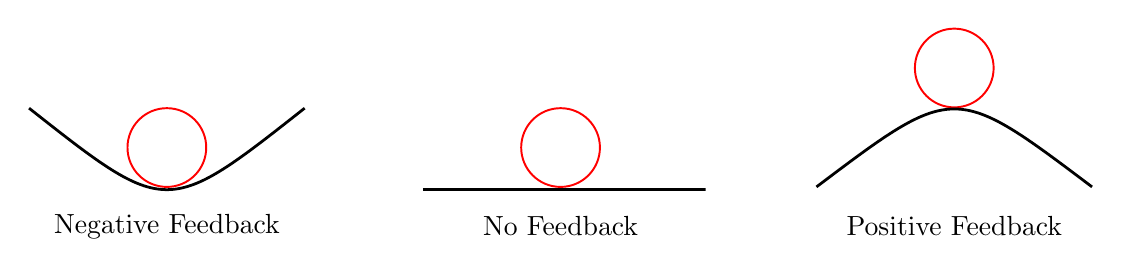
\begin{tikzpicture}[scale = 1]
        %%%%%%%%% ball in bowl %%%%%%%%%%%%%%%%%
        \draw[color = red, line width = 0.7pt] (0,0) circle(0.5);
        \draw[line width=1.pt] (-1.75, 0.5) .. controls(0,-0.88) .. (1.75, 0.5);  
        \node at (0, -1.0) {Negative Feedback};
        %%%%%%%%% flat plane ball %%%%%%%%%%%%%%  
        \draw[color = red, line width = 0.7pt] (5+0,0) circle(0.5);
        \draw[line width=1.pt] (5-1.75, -0.53) .. controls(5+2,-0.53) .. (5+1.75, -0.53);
        \node at (5, -1.0) {No Feedback};
        %%%%%%%%%% ball on bowl %%%%%%%%%%%%%%%%%
        \draw[color = red, line width = 0.7pt] (10,1.01) circle(0.5);
        \draw[line width=1.pt] (10-1.75, -0.5) .. controls(10,0.82) .. (10+1.75, -0.5);
        \node at (10, -1.0) {Positive Feedback};
    \end{tikzpicture}   
    \caption{An example of various feedback loops. Consider a ball at rest on various surfaces that is suddenly displaced by a small amount in one direction (we are looking at a cross section). On the left, a ball is in a bowl, and when displaced from either side, the ball will roll back and forth, always returning to the center of the bowl. In the middle image, we have a ball on a flat surface. When displaced, it simply changes locations. On the right, we have a ball balanced on a bowl. If displaced slightly, its balance is upset, and it will roll down the bowl faster and faster and faster.}
    \label{fig:feedback}
    \end{figure}

    This may have been a lengthy aside but one that is important. For example, if we look at feedback in the context of our dark earth model, then we need to consider a few situations. For instance, consider what would happen if the surface temperature drops to below its equilibrium temperature. According to Stefan's Law (Eq.~\ref{eq:stefan_law}), then the rate at which the earth energy would be radiated away would also drop, cooling itself, thus returning to equilibrium. This is an example of negative feedback.

    \begin{exercise}
        Find two examples of feedback loops on your own: one positive and one negative.
        \label{ex:feedback_loops}
    \end{exercise}

    % subsubsection feedback (end)


    \subsection{The Shiny Earth Model} % (fold)
    \label{sub:shiny_earth}
   
    To motivate why we need to refine our model of the earth, we should consider Figure~\ref{fig:earthrise}.

    \begin{figure}[hb!]
        \centering
        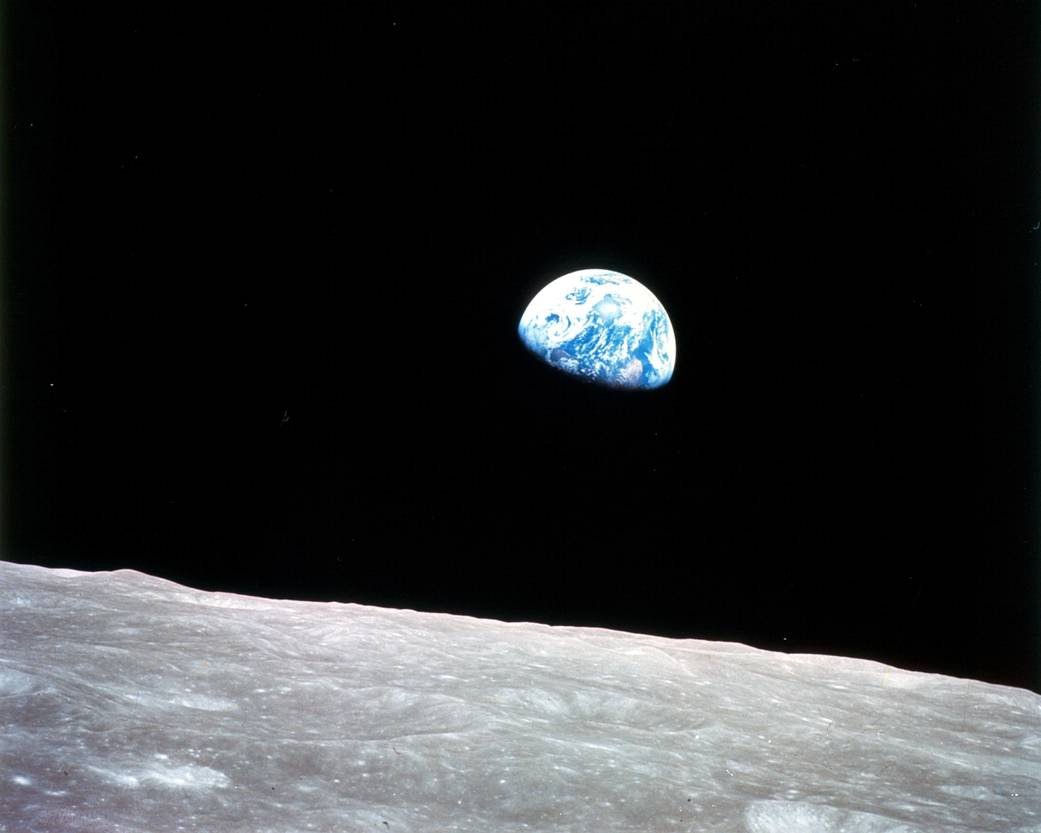
\includegraphics[width = 0.6\textwidth]{earthrise.jpg}
        \caption{The famous ``Earthrise'' photo taken during the Apollo 8 lunar mission. Image taken from NASA.}
        \label{fig:earthrise}
    \end{figure}

    If the earth, as we assumed in Sec.~\ref{sub:dark_earth}, absorbed all incident light, we would not see an image like the Apollo 8 astronauts did; rather we would see nothing as the earth would appear black.  From our everyday experience, we know some objects (e.g. clouds, ice, snow, etc.) reflect a large fraction of the light incident upon them (see Table~\ref{tab:albedo}), again illustrated in Figure~\ref{fig:earthrise}. The reflectivity of an object averaged over the entire surface is known as its \textbf{albedo}, and we will denote it as $A$ in equations in this text. The earth reflects roughly 30\% of the sun's incident light, meaning that $A = 0.30$, and the remaining light is absorbed \citep{schroeder1999introduction,thorndike1976energy} Consequently, we must modify Eq.~(\ref{eq:earth_temp}) so that this is taken into account. It is a small correction yet important and is given below.
    \begin{align}
        T = \left( \frac{(1-A) \mathcal{S}}{4 \sigma} \right)^{1/4} = \left( \frac{(0.70) \cdot \SI{1370}{\watt/\meter^2}}{4 \cdot \SI{5.67e-8}{\watt/(\meter^2 \kelvin^4)} } \right)^{1/4} = \SI{255}{\kelvin}
        \label{eq:shiny_earth_temp}
    \end{align}
    We found our new equilibrium temperature is a frigid \SI{255}{\kelvin} (\SI{-18}{\celsius}) which is much colder than we did before. The result is worse if we consider the feedback loops as related to the earth's albedo. Consider a slight drop in temperature on earth, below its equilibrium. This will lead to more snow---which reflects more light from the sun---which consequently increasing the albedo. The larger albedo lowers the equilibrium temperature further---as we just saw---leading to more snow being formed. So in this example, the feedback loop is positive. Conversely, a slight warming of earth  will melt snow and glaciers, reflecting less light, and decreasing the albedo. This will cause an increase in the earth's equilibrium temperature which is also a positive feedback loop. The big takeaway is that the system appears to be unstable.

    \begin{table}[ht]
    \centering
    \begin{tabular}{|p{5cm}|p{6cm}|}
        \hline
        \textbf{Object}     & \textbf{Reflectivity (percent)}\\
        \hline
        Clouds & 20--70 (depends on type and thickness) \\
        Open Water  & 3--8 \\
        Open Water (polar regions) & 25 (due to larger angle of incidence) \\
        Snow and ice   & 30--70 \\
        Arable land \& Coniferous forest & 10--15 \\
        Deciduous forest  & 18   \\
        Desert & 30  \\
        \hline
    \end{tabular}
    \caption{Reflectivity of various surfaces on Earth, all of which contribute to the earth's overall albedo \citep{thorndike1976energy}. The percentages tell you how much incident light is reflected for a given surface.}  
    \label{tab:albedo}     
    \end{table}


   %%%%%%%%%%%%%%%%%%%%%
   %% ATMOSPHERE
   %%%%%%%%%%%%%%%%%%%%% 
    
   \section{The Atmosphere} % (fold)
   \label{sec:the_atmosphere}
	
	\subsection{Modeling an Interacting Atmosphere}
    
    In the previous section, we found that with a more realistic model of the earth, the average surface temperature will be a chilly \SI{255}{\kelvin} (\SI{-18}{\celsius}) by taking into account the reflectivity of the earth's surface and atmosphere. However, we have yet to consider how the atmosphere interacts with the incident sunlight on the whole which is what we will do next.

    \begin{figure}[ht]
        \centering 
        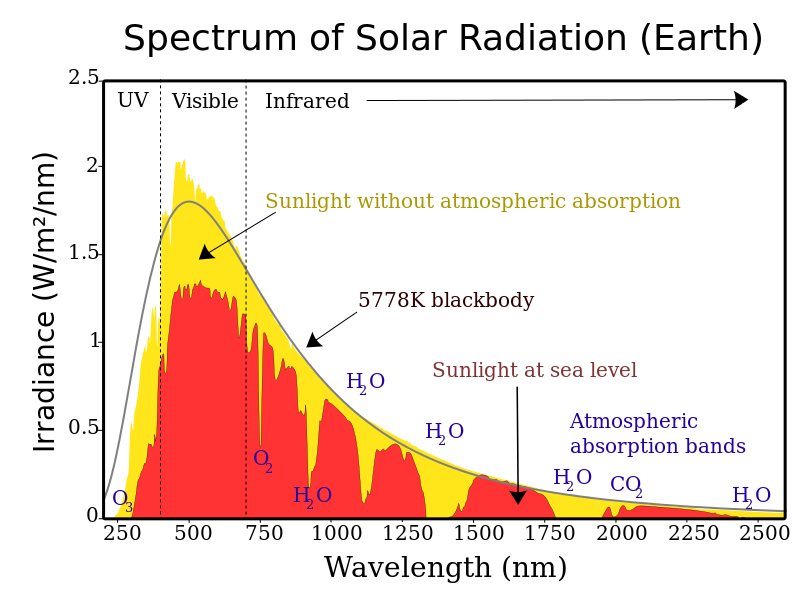
\includegraphics[width = 0.6\textwidth]{Solar_spectrum_en.png}
        \caption{A spectrum showing the actual solar distribution, compared to the blackbody distribution (c.f. Figure~\ref{fig:sun_bb}), as well as the sunlight that reaches sea level. This is a figure with a lot of information. Take time to look over it carefully and understand it. Taken from Wikipedia.}
        \label{fig:solar_spec}
    \end{figure}

    The earth's atmosphere is largely transparent to the incident solar spectrum (in the visible region as well as the near ultraviolet and near infrared light). However, we are going to consider what happens to the absorption of ultraviolet and infrared radiation in the atmosphere and the processes they are responsible for creating \citep{schroeder1999introduction,thorndike1976energy}. We will consider these in turn.

    \subsection{Interaction of UV Light} % (fold)
    \label{sub:uv_light}
    
    % subsection uv_light (end)
    If we look at the UV-radiation first, we should note that light below \SI{300}{\nm} is harmful to humans and most living creatures \citep{thorndike1976energy} This is the type of light that causes sunburns as well as damages the DNA of living organisms. In addition to this, these wavelengths of light are capable of breaking the chemical bonds that are found in living matter. Fortunately for us, wavelengths of light shorter than \SI{180}{\nm} are absorbed heavily by molecular oxygen in the upper-most layer of the atmosphere (called the \textbf{ionosphere}) nearly \SI{100}{km} above the earth's surface \citep{thorndike1976energy}. Wavelengths of light between \SI{180}{\nm} and \SI{290}{\nm} are less strongly absorbed and penetrate through the ionosphere and the mesosphere (which is below the ionosphere) where it is eventually absorbed by the stratosphere by molecular oxygen gas and ozone\footnote{
        Ozone is an important gas that is found high in the earth's atmosphere. It plays an important role for life on Earth as it acts as a filter by absorbing harmful UV-rays \citep{spiro2012chemistry}.
        }
    (O$_2$ and O$_3$ respectively). Light with wavelengths larger than \SI{290}{\nm} are only weakly absorbed: only around 20\% are absorbed before reaching the earth's surface.

    This ultraviolet light also causes chemical processes to occur due to its high energy. Ozone in the atmosphere is inherently unstable; despite this, it has a long lifetime in the atmosphere before it breaks down. However, this breakdown can be accelerated by the introduction of other chemicals in the atmosphere. In 1974, Mario Molina and F. Sherwood Rowland (who ended up winning the Nobel Prize in Chemistry in 1995 for this work) realized that a chlorine atoms (Cl) are very effective at breaking down ozone in the atmosphere. A certain class of gaseous molecules, called \textbf{chlorofluorocarbon molecules (CFC)}---which are made up of a carbon atom surrounded by chlorine and fluorine atoms---don't undergo any reaction until they reach the upper atmosphere. While in the upper atmosphere, the energetic UV-light break the carbon-chlorine bond, allowing the chlorine atom to react with ozone in the atmosphere, breaking it down. Eventually it was discovered that there was a large ``hole'' in ozone over the South Pole. By ``hole'' we mean that the concentration of ozone was significantly lower in the atmosphere than other parts of the world.

    This was so problematic that soon after Molina and Rowland's work, international governments came together to ban the use of CFCs by signing the Montreal, London, Copenhagen, and Vienna protocols in 1987, 1990, 1992, and 1995, respectively \citep{spiro2012chemistry} Their work is a shinning example of the ways the scientific method can unify people of diverse backgrounds to address global challenges.


    \subsection{Interaction of IR Light} % (fold)
    \label{sub:ir_light}

    While the earth's atmosphere is largely transparent to infrared radiation produced by the sun, it is very much opaque the earth's re-radiation. In fact, if you were to look at the earth from outer space with an eye that is only sensitive to infrared light, what you see is mostly the atmosphere and not the surface because none of that light is able to make it through the atmosphere without being absorbed. The equilibrium temperature we calculated in Sec.~\ref{sub:shiny_earth} of \SI{255}{\kelvin} is (roughly) the temperature of the upper atmosphere \citep{schroeder1999introduction} 

    Just like the sun can be modeled as a blackbody that produces the largest amount of solar radiation in the visible spectrum, the earth acts as a blackbody that peaks in the infrared light. However, this frequency of light that the earth emits (at a temperature of \SI{294}{\kelvin}) is largely absorbed by various gases in the atmosphere. In other words, the heat radiated by the earth's surface will not disperse directly into space but will be absorbed by the atmosphere. When the atmosphere absorbs this energy, the atmosphere will warm and re-radiate some of this energy back to earth in the form of infrared light, also warming the earth's surface. Thus, the atmosphere acts as a sort of blanket that keeps the earth's surface warmer than it would be otherwise. This phenomena is called the \textbf{greenhouse effect} and is important for maintaining life here on earth by keeping the earth at more mild temperature.

    \begin{figure}[ht]
        \centering
        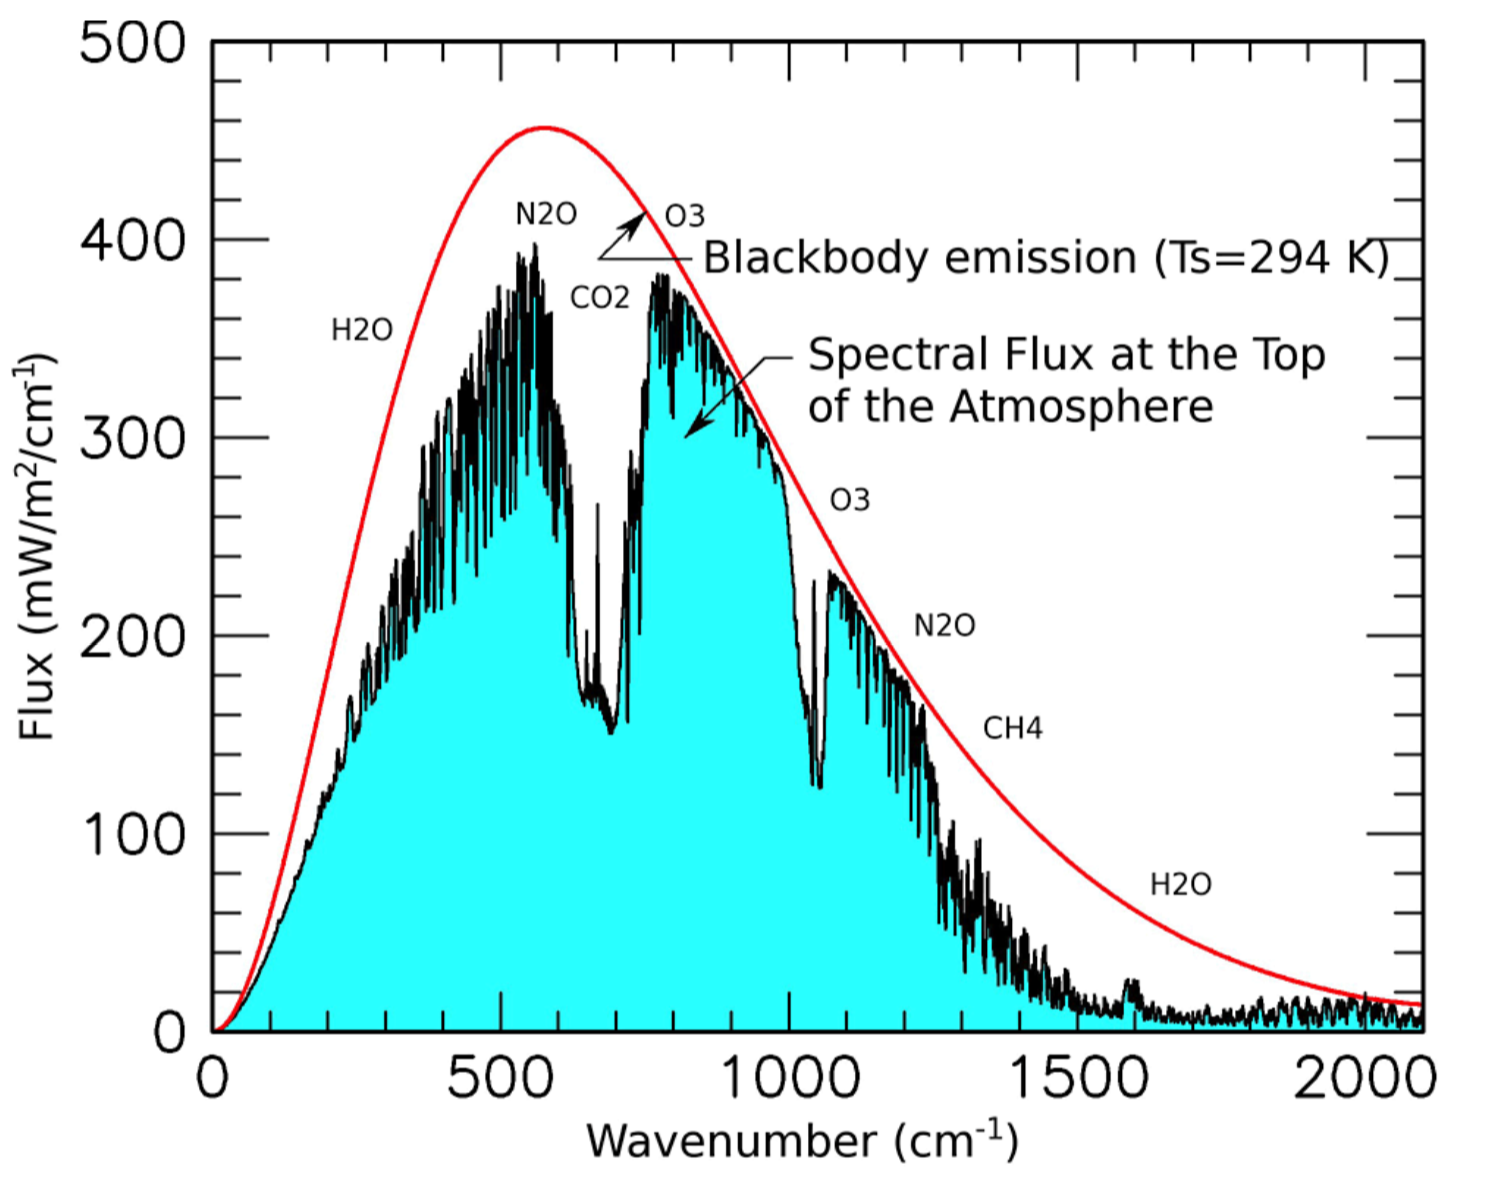
\includegraphics[width = 0.6\textwidth]{vibs_greenhouse.png}
        \caption{The blackbody spectrum of the earth (red) compared to what is measured (blue). This discrepancy comes from the rotational and vibrational excitations of the greenhouse gases (e.g. water, methane, etc.). See Appendix~\ref{app:symmetry}. The gap between the red and the blue is where the various greenhouse gases absorbed energy.}
        \label{fig:earth_bb}
    \end{figure}

    The gases in the atmosphere that are responsible for the absorption of the earth's infrared radiation are called \textbf{greenhouse gases}. Some examples of these include water, carbon dioxide, nitrous oxide, and methane.\footnote{In fact, water is the earth's largest greenhouse gas, however you don't hear about it in the news as there isn't anything we can really do about releasing water into the atmosphere. Carbon dioxide is another story on the other hand as we can control how much carbon dioxide is released through the burning of fossil fuels.} As you probably expect, different gases have a different impact on the greenhouse effect. The measure of how well a greenhouse gas can trap heat is characterized by the \textbf{Global Warming Potential (GWP)}. GWP is characterized by the following criteria:
    \begin{enumerate}
        \item The absorption of infrared radiation by a given species,
        \item The spectral location of absorbing wavelengths. This means, where on Figure~\ref{fig:earth_bb} does the light absorb. Is it closer to where the red curve peaks or closer to the tail end? 
        \item The atmospheric lifetime of the chemical species.
    \end{enumerate}
    The standard GWP reference is carbon dioxide. The GWP for nitrous oxide ({$\rm N_2O$}) and methane ({$\rm CH_4$}), over a time period of twenty years, is 268 and 86, respectively. 
    
    It's important to explicitly note that not all gases are greenhouse gases. Only gases that absorb the infrared radiation produced by the earth through rotations and vibrations act as greenhouse gases. For a much more thorough description of how and why certain molecules behave as greenhouse gases, I would strongly encourage you to read Appendix~A. 
    
    % subsubsection ir_light (end)

    \subsection{The Shell-Atmosphere Model} % (fold)
    \label{sub:shell_atm}

    The greenhouse effect is essential for maintaining the earth's surface temperature at a reasonable level. To make a simple model, as we have done multiple times in this chapter already, we assume a ``shell of atmosphere'' that is a single layer above the earth's surface that is transparent to the sun's visible light but opaque to the earth's infrared light. Since the shell is transparent to the sun, the energy flowing into the earth would be the same as if the shell were not there. Because all of the energy radiated by the earth is stopped by the shell, it follows that the shell would have the temperature that we calculated in Sec.~\ref{sub:shiny_earth}, namely \SI{255}{\kelvin}. The shell, on the other hand, will not only radiate energy to space but will radiate some back to the earth's surface. A good illustration of this description is found in Figure~\ref{fig:greenhouse_effect}. 

    \begin{figure}[ht]
        \centering 
        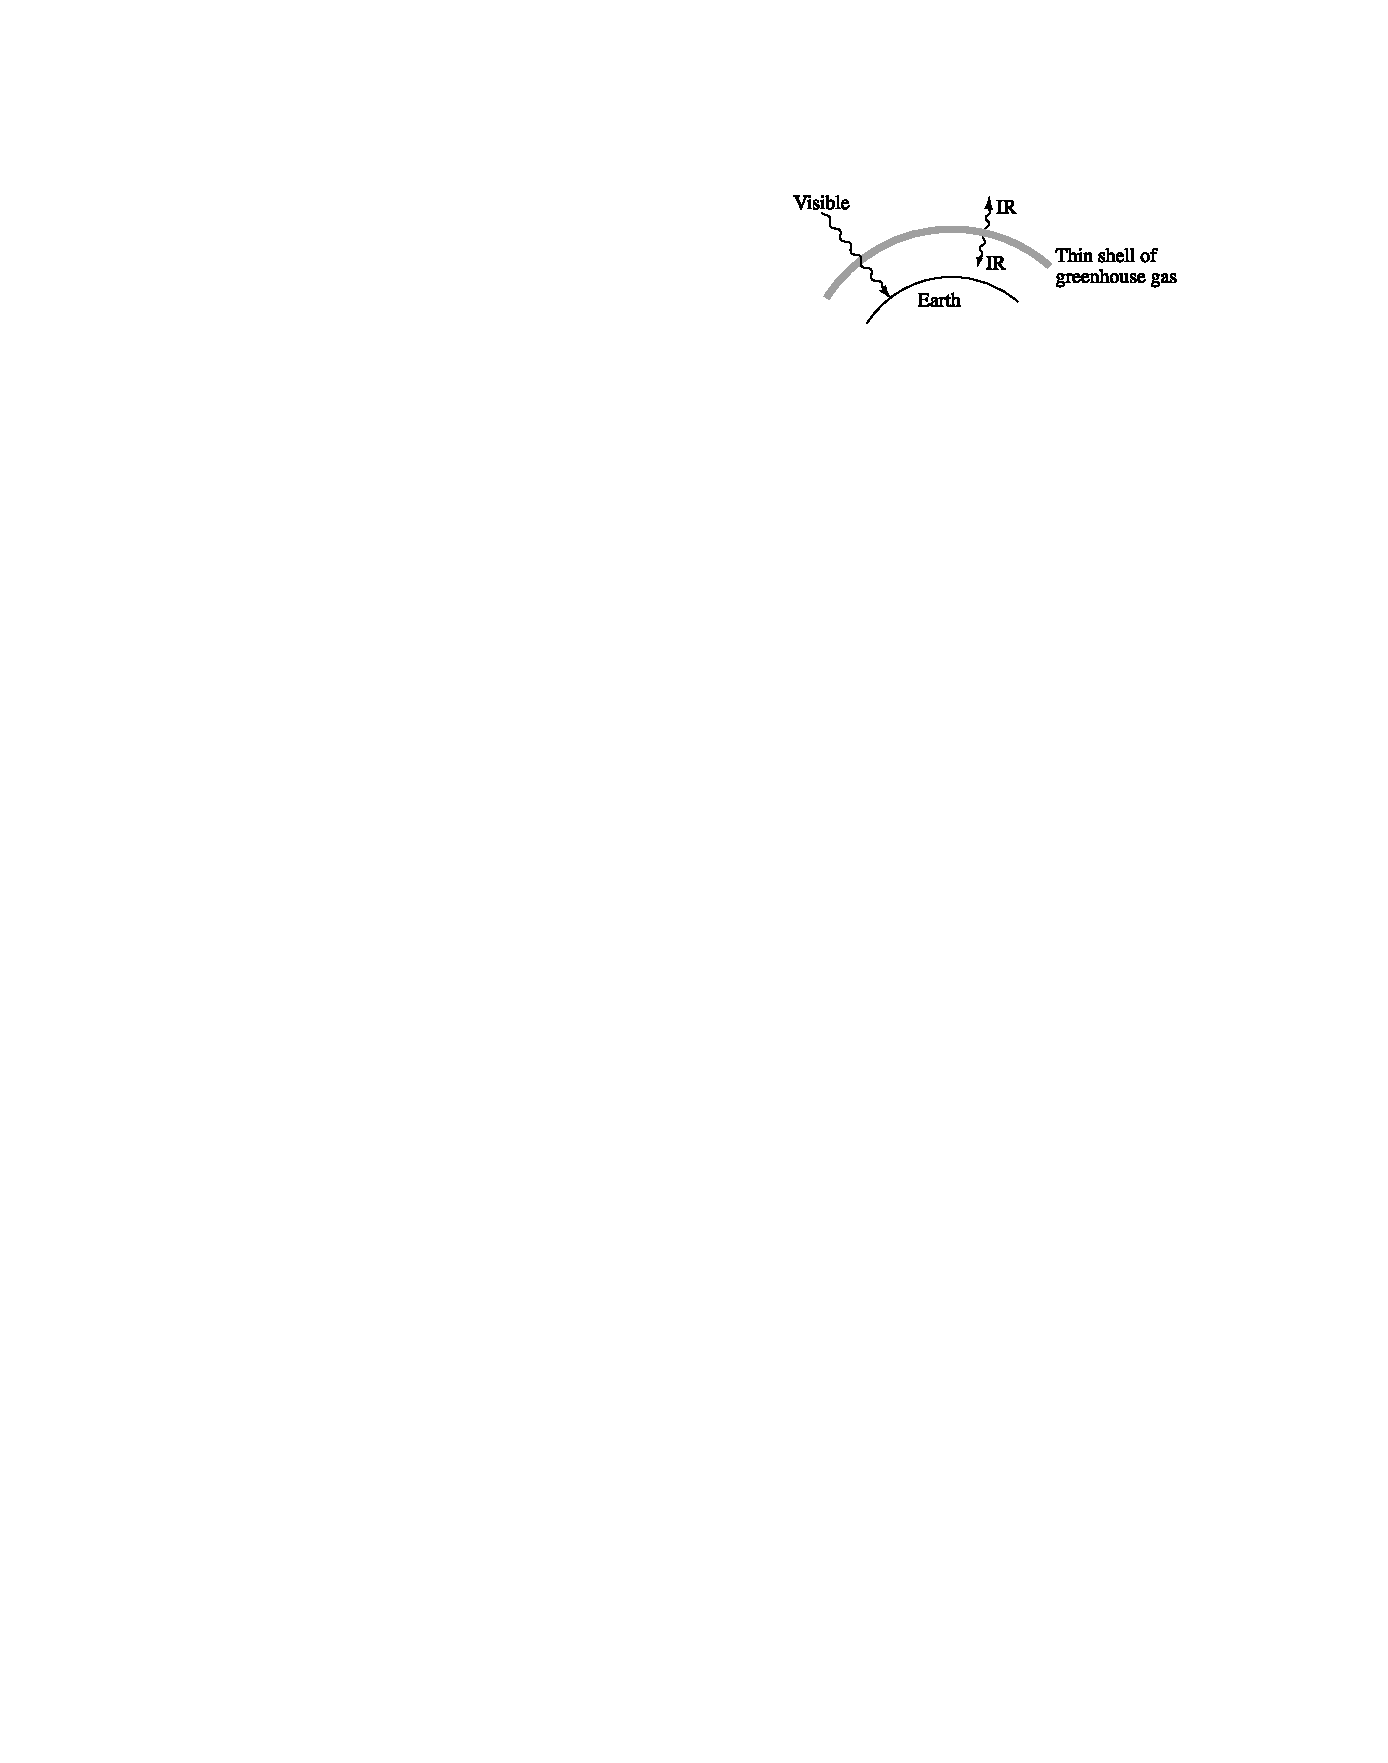
\includegraphics[width = 0.6\textwidth]{greenhouse_effect.pdf}
        \caption{A simple model of the earth's atmosphere as a thin shell. Equilibrium requires that the earth's surface receive as much energy from the atmosphere as the sun. Taken with permission from \emph{Quantum Physics} (2010) by John S. Townsend \citep{townsend2010baby}} 
        \label{fig:greenhouse_effect}
    \end{figure}

    Consequently, the energy that the earth will receive will be twice that of the ``no shell'' calculation we had in Sec.~\ref{sub:shiny_earth}. Thus, we would expect the temperature to be 
    \begin{align}
        T = 2^{1/4} \cdot \SI{255}{\kelvin} = \SI{303}{\kelvin}.
    \end{align}
    This is a temperature of \SI{30}{\celsius} which is much more pleasant to live in! This temperature we calculated is a little higher than what scientists measure experimentally, but then again we made a very simple model of an atmosphere. The real atmosphere isn't a single, perfectly opaque layer, but this example brings home the point that the greenhouse effect is important to maintaining life by creating a warmer environment. This model predicts that the more IR-absorbing material (e.g. carbon dioxide and methane) there is in the atmosphere, the higher the surface temperature of the earth. In fact, this can get very out of hand, causing a planet to get extremely hot. This is called a runaway greenhouse effect and is an example of a positive feedback loop. To see what happens and how this actually works, I encourage you to work out Exercise~\ref{ex:venus} and look at Figure~\ref{fig:earth_stability}.

    \begin{figure}[hb]
    \centering
      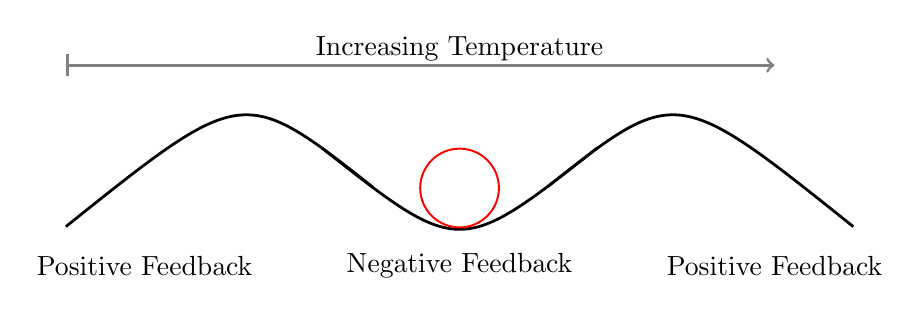
\begin{tikzpicture}[scale = 1]
        \draw[line width=1.pt] (0., -0.5) .. controls(7.75-5.5,1.3) .. (3.9, 0);
        \node at (1, -1.0) {Positive Feedback};
        %%%%%%%%% ball in bowl %%%%%%%%%%%%%%%%%
        \draw[line width=1.pt] (5+ -1.75, 0.5) .. controls(5+0,-0.88) .. (5+1.75, 0.5); 
        \node at (5, -1.0) {Negative Feedback};
        %%%%%%%%% flat plane ball %%%%%%%%%%%%%%  
        \draw[color = red, line width = 0.7pt] (5+0,-0.010) circle(0.5);
        %%%%%%%%%% ball on bowl %%%%%%%%%%%%%%%%%
        \draw[line width=1.pt] (6.11, 0) .. controls(7.75,1.3) .. (10, -0.50);
        \node at (9., -1.0) {Positive Feedback};
        \draw[|->, color=gray, line width = 1] (0, 1.55) -- (9, 1.55);
        \node at (5,1.755) {Increasing Temperature};
    \end{tikzpicture}
    \caption{A simplified view of the feedback processes of the earth's surface temperature. If it gets too cold, there will be a runaway albedo effect much like the ice age where more and more ice forms on the Earth. This is an example of positive feedback. As the concentration of the greenhouse gases increases, there is a point of no return and we have a runaway greenhouse effect, i.e. positive feedback. Luckily we live in a ``sweetspot'' where these forces seem to cancel each other out. }
    \label{fig:earth_stability}
    \end{figure}

    \begin{exercise}
        The planet Venus is different than Earth in several respects; First, it is 30\% closer to the sun. Next, it has thick clouds that reflect 77\% of the incident sunlight. Finally, its very thick atmosphere is much more opaque to infrared light than the earth's. Given the solar constant for Venus, which we will denote by $\mathcal{V}$ (rather than Earth's solar constant $\mathcal{S}$), takes on a value of $\mathcal{V} = \SI{2796}{\watt/(\meter^2 \kelvin^4)}$:
        \begin{enumerate}[(a)]
            \item Calculate the surface temperature of Venus if it did not reflect any incident light.
            \item Estimate the surface temperature taking Venus' albedo into account.
            \item The atmosphere of Venus absorbs roughly 70 times the amount of infrared light of that of Earth's atmosphere. We can model this with 70 successive atmospheric shells like we did in Sec.~\ref{sub:shell_atm} with \underline{each shell at a different equilibrium temperature.} The temperature of the top layer will be what you found in part (b). The next layer is warmer by a factor of $2^{1/4}$. The layer below that is warmer by a smaller factor. Keep working your way down until you see a pattern.

            Use this to estimate the surface temperature of Venus. The measured surface temperature of Venus is $\SI{740}{\kelvin}$; how does your answer compare? This is a good illustration of the runaway greenhouse effect.
        \end{enumerate}
        Note: this is a challenging problem! Don't worry if you don't get it immediately! 
        \label{ex:venus}
    \end{exercise}
    
    % subsection the_atmosphere (end)    

    % section the_atmosphere (end)

%%%%%%%%%%%%%%%%%%%%%%%%%%%%%%%%
%% CONNECT TO REST OF TEXTBOOK
%%%%%%%%%%%%%%%%%%%%%%%%%%%%%%%%

\section{Greenhouse Gases in Asia} % (fold)
\label{sec:gg_in_asia}

\subsection{Gross versus Per Capita GHG Emissions}

After seeing the potential for the greenhouse effect to raise the surface temperature, we should look at carbon dioxide emissions around the world. Specifically, we are going to focus on Asia's emissions. The Asian economy is made up of more than 4.5 billion people which is significantly more than half of the world's population. In addition to this, Asia is the largest and fastest growing economic region in the world, according to the International Monetary Fund. In addition to this, the Organization for Economic Cooperation and Development (OECD) projects that Asia will remain the fastest growing economic region in the world through 2030. All the while, the population and energy demands of the region (and world) will increase. Economic growth and greenhouse gas emissions---specifically carbon dioxide---have been linked together \citep{saidi2015impact}.

\begin{figure}[ht!]
    \centering
    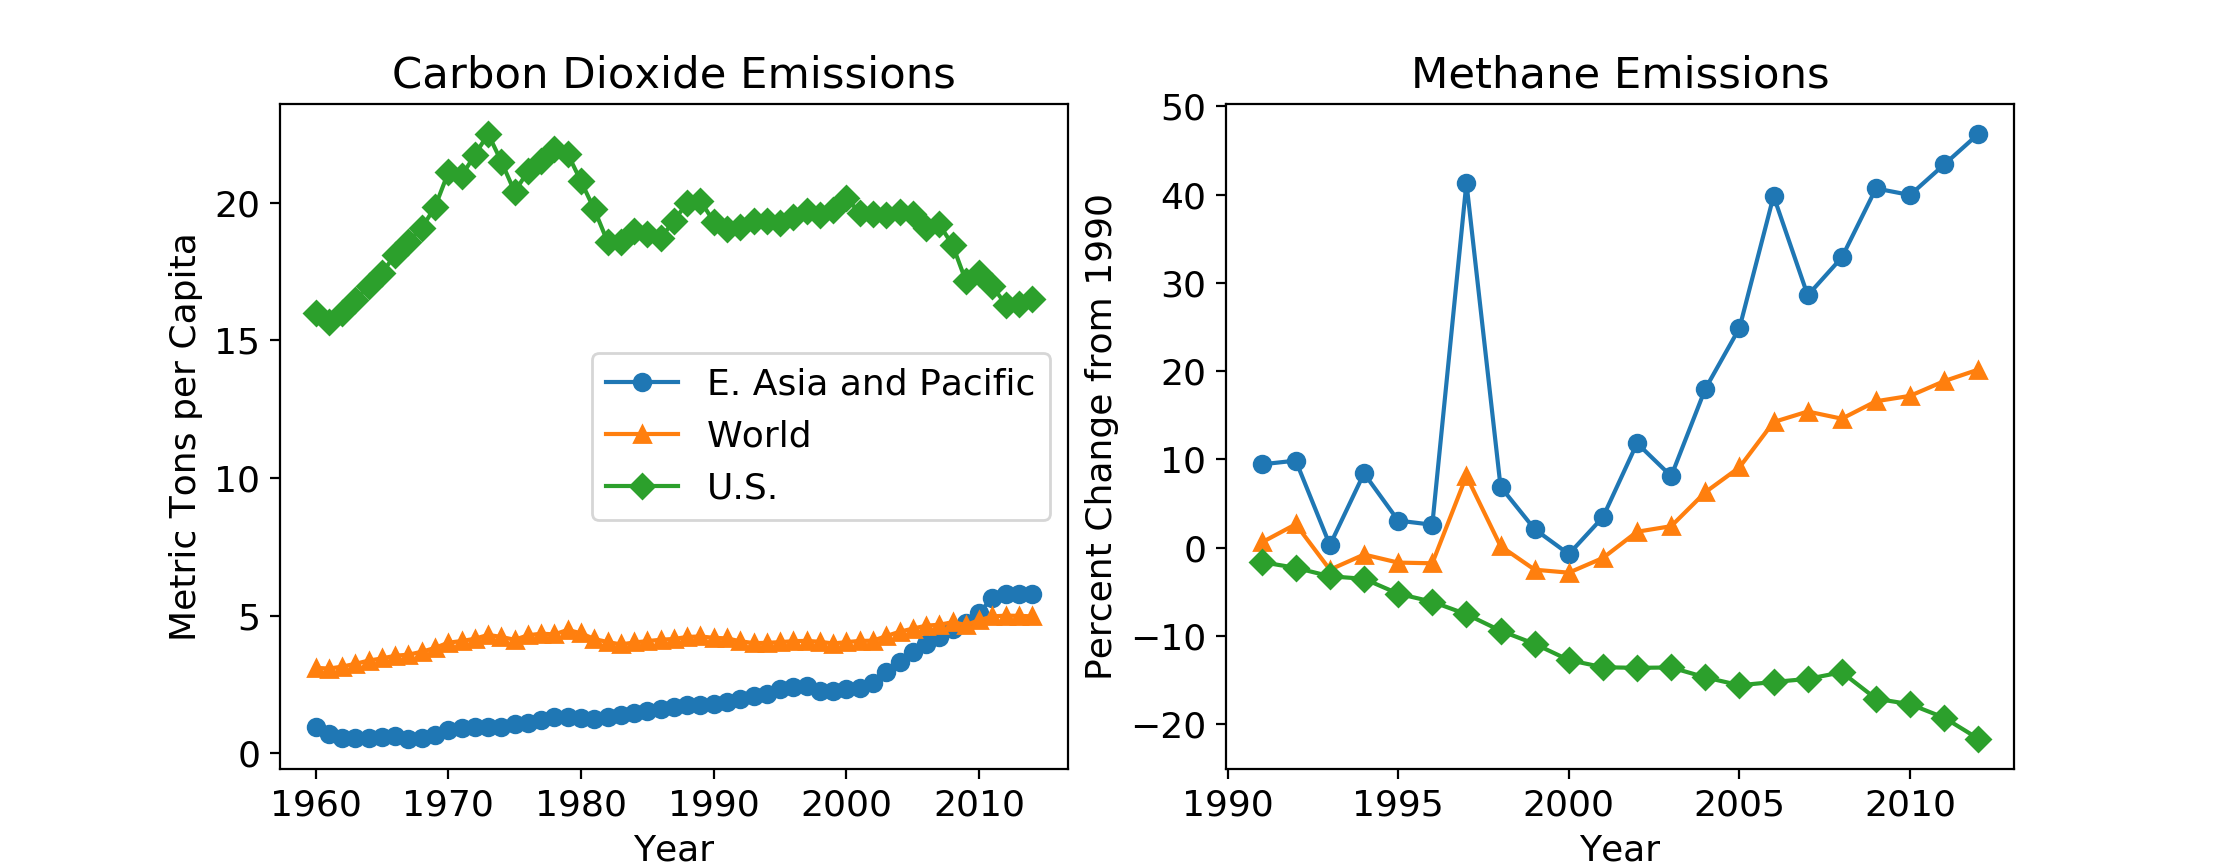
\includegraphics[width = \textwidth]{emissions3.png}
    \caption{The relative emissions of East Asian and Pacific countries (excluding the high income population) compared to the world taken as a whole. Data taken from the World Bank and is current up to 2014 \citep{WBco2,WBmethane}.} 
    \label{fig:asia_emissions}
\end{figure}

As you might expect, a rapidly growing economy needs to produce a large amount of energy. Currently, a cheap and convenient form of energy is \textbf{fossil fuels}, which are natural fuels that formed millions of years ago from the remains of organisms. Some examples of fossil fuels are coal, oil, and natural gas (methane). Fossil fuels are burned in order to release energy, in the form of heat, into their surroundings allowing work to be done. However, when fossil fuels are burned, they release carbon dioxide and water into the atmosphere. Now we can make a prediction. Since Asia has and, recently, has had the fastest growing economy in the world, we would expect the emissions of the region to be rising faster compared to the rest of the world. This is exactly what we see in Figure~\ref{fig:asia_emissions}. Since the early 2000's, there has been a steady and relatively constant increase in the amount of both carbon dioxide and methane into the atmosphere. In comparison to the rest of the world, East Asia and the Pacific are releasing significantly more carbon dioxide per person and methane per year into the atmosphere. However, Asia---as a continent---has a significantly higher population than the the rest of the world.

This release of greenhouse gases will, as we saw in our toy model, lead to an increase in average surface temperature of the earth. This change will affect many aspects of the earth.  This is why people are concerned about releasing greenhouse gases into the atmosphere. When the average surface temperature of the earth warms, it causes large problems in ecosystems. This phenomena is called \textbf{climate change} and is at the forefront of international and scientific communities because of its potential consequences. Climate change and its consequences will be of central focus to the rest of this book.

\begin{figure}[hb!]
    \centering
    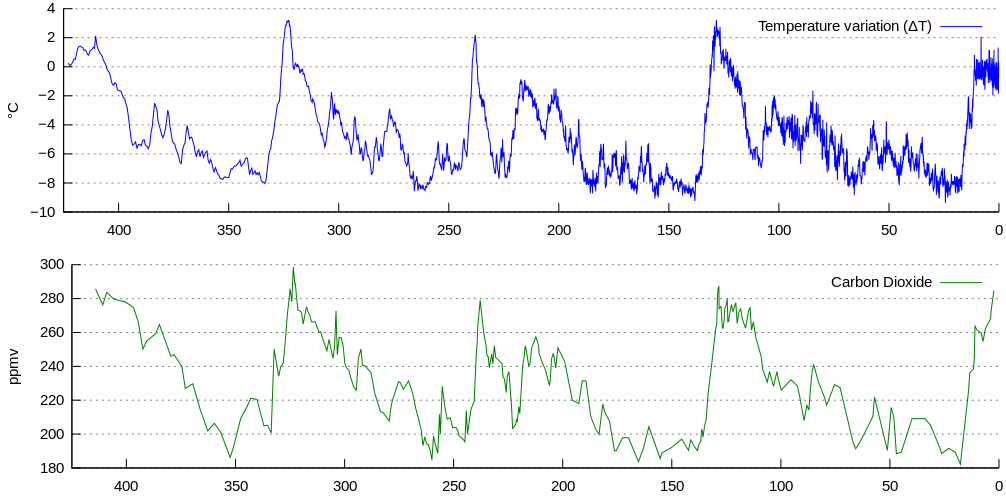
\includegraphics[width = 0.8\textwidth]{Vostok_Petit_data.png}
    \caption{Correlation between the temperature of the earth with the concentration of carbon dioxide over a timescale of 420,000 years. Data is taken from the Vostok ice core in  The current concentration of carbon dioxide is over 400 parts per million (ppm). Taken from Wikipedia.}
    \label{fig:ice_core}
\end{figure}

% section greenhouse_gases_in_asia (end)

%%%%%%%%%%%%%%%%%%%%%%%
%% CONCLUSION 
%%%%%%%%%%%%%%%%%%%%%%%

\section{Conclusion} % (fold)
\label{sec:conclusion}

The earth, although it may seem large to us humans, is merely a pale blue dot when compared to the solar system as a whole. Almost the entirety of Earth's energy comes from the sun. In fact, at the top of the atmosphere, we receive \SI{1370}{\watt} of power for every square meter, or one solar constant. With this, an important greenhouse effect, and little else, over the course of billions of years, life has managed to not only start but thrive. Some of the organisms that lived and died millions of years ago have converted into fossil fuels  by geologic processes. 

Today, almost the entirety of the world is dependent on burning these fossil fuels for energy, to fuel growing economies, to power our lights, and even produce the food we eat. However, extracting and burning these fossil fuels has and will continue to release potent greenhouse gases into our atmosphere--contributing to one of the most pervasive positive feedback loops of our generation: global climate change. Because fossil fuels are so integral to the world's infrastructure today, we should look at them more closely. This is the topic of our next chapter.

% section conclusion (end)


%%%%%%%%%%%%%%%%%%%%%%%%%%%%%%%%%%%%%
%% APPENDIX: SYMMETRY OF MOLECULES
%%%%%%%%%%%%%%%%%%%%%%%%%%%%%%%%%%%%%
\newpage
\section*{\label{app:symmetry}{\LARGE{Appendix A:}}\\The Symmetry of Molecules and Greenhouse Gases}

    In this appendix we are going to focus on how various molecules are able to move around. Specifically, we will look at how molecules translate, rotate, and---most importantly---vibrate. Now why do we care? How molecules are able to move plays a fundamental role in what type and how much energy they absorb. We will learn why some gases it the atmosphere are greenhouse gases and some are not.

    In order to make this appendix tractable, I'm assuming that you have some basic chemistry background already.

    \section*{Chemical Bonding} % (fold)
    \label{sec:bonding}
            
    Molecules, quite simply, are atoms that are bonded together via \textbf{chemical bonds}. Chemical bonds are the links between atoms \citep{atkins2014physical} There are a few different types of common, chemical bonds that we see around us in Nature:
    \begin{enumerate*}[(1)]
        \item covalent bonding,
        \item ionic bonding, and
        \item metallic bonding.
    \end{enumerate*}
    In this appendix, we are mainly going to focus molecules that are held together through covalent bonds; another name for these molecules are covalent compounds. \textbf{Covalent bonds} are bonds in molecules where different atoms will share pairs of electrons in order to reduce their energies. For example, water, methane, and carbon dioxide have each of their respective atoms bonded together like this.

    When molecules are formed, their shape is determined by minimizing the repulsion from the negatively charged electrons surrounding the various atoms in the molecule \citep{atkins2014physical} This comes about from various lone pairs of electrons that originate with covalently-bonded molecules. Lone pairs of electrons are assumed to be more repulsive than bonded atoms. Because of this, molecules take the shape as to maximize the separation of these lone pairs.\footnote{For an understanding of how these molecules take these shapes, I recommend reading any general chemistry textbook or a good online resource like \texttt{www.khanacademy.org/science/chemistry/chemical-bonds} about valence-shell electron pair repulsion (VSEPR) as well as Lewis Structures.} 

    We will look at the geometric shapes a few different molecules that will frequently appear, except for sulfur hexafluoride, and are relevant in this text: carbon dioxide (CO$_2$), water (H$_2$O), methane (CH$_4$), and sulfur hexafluoride (SF$_6$). All four of these molecules are \textbf{polyatomic molecules}, meaning that there is more than one type of atom present, e.g. hydrogen and oxygen constitute the elements of water, sulfur and fluorine are the elements found in sulfur hexafluoride, etc. 

    \begin{figure}[ht]
        \centering
        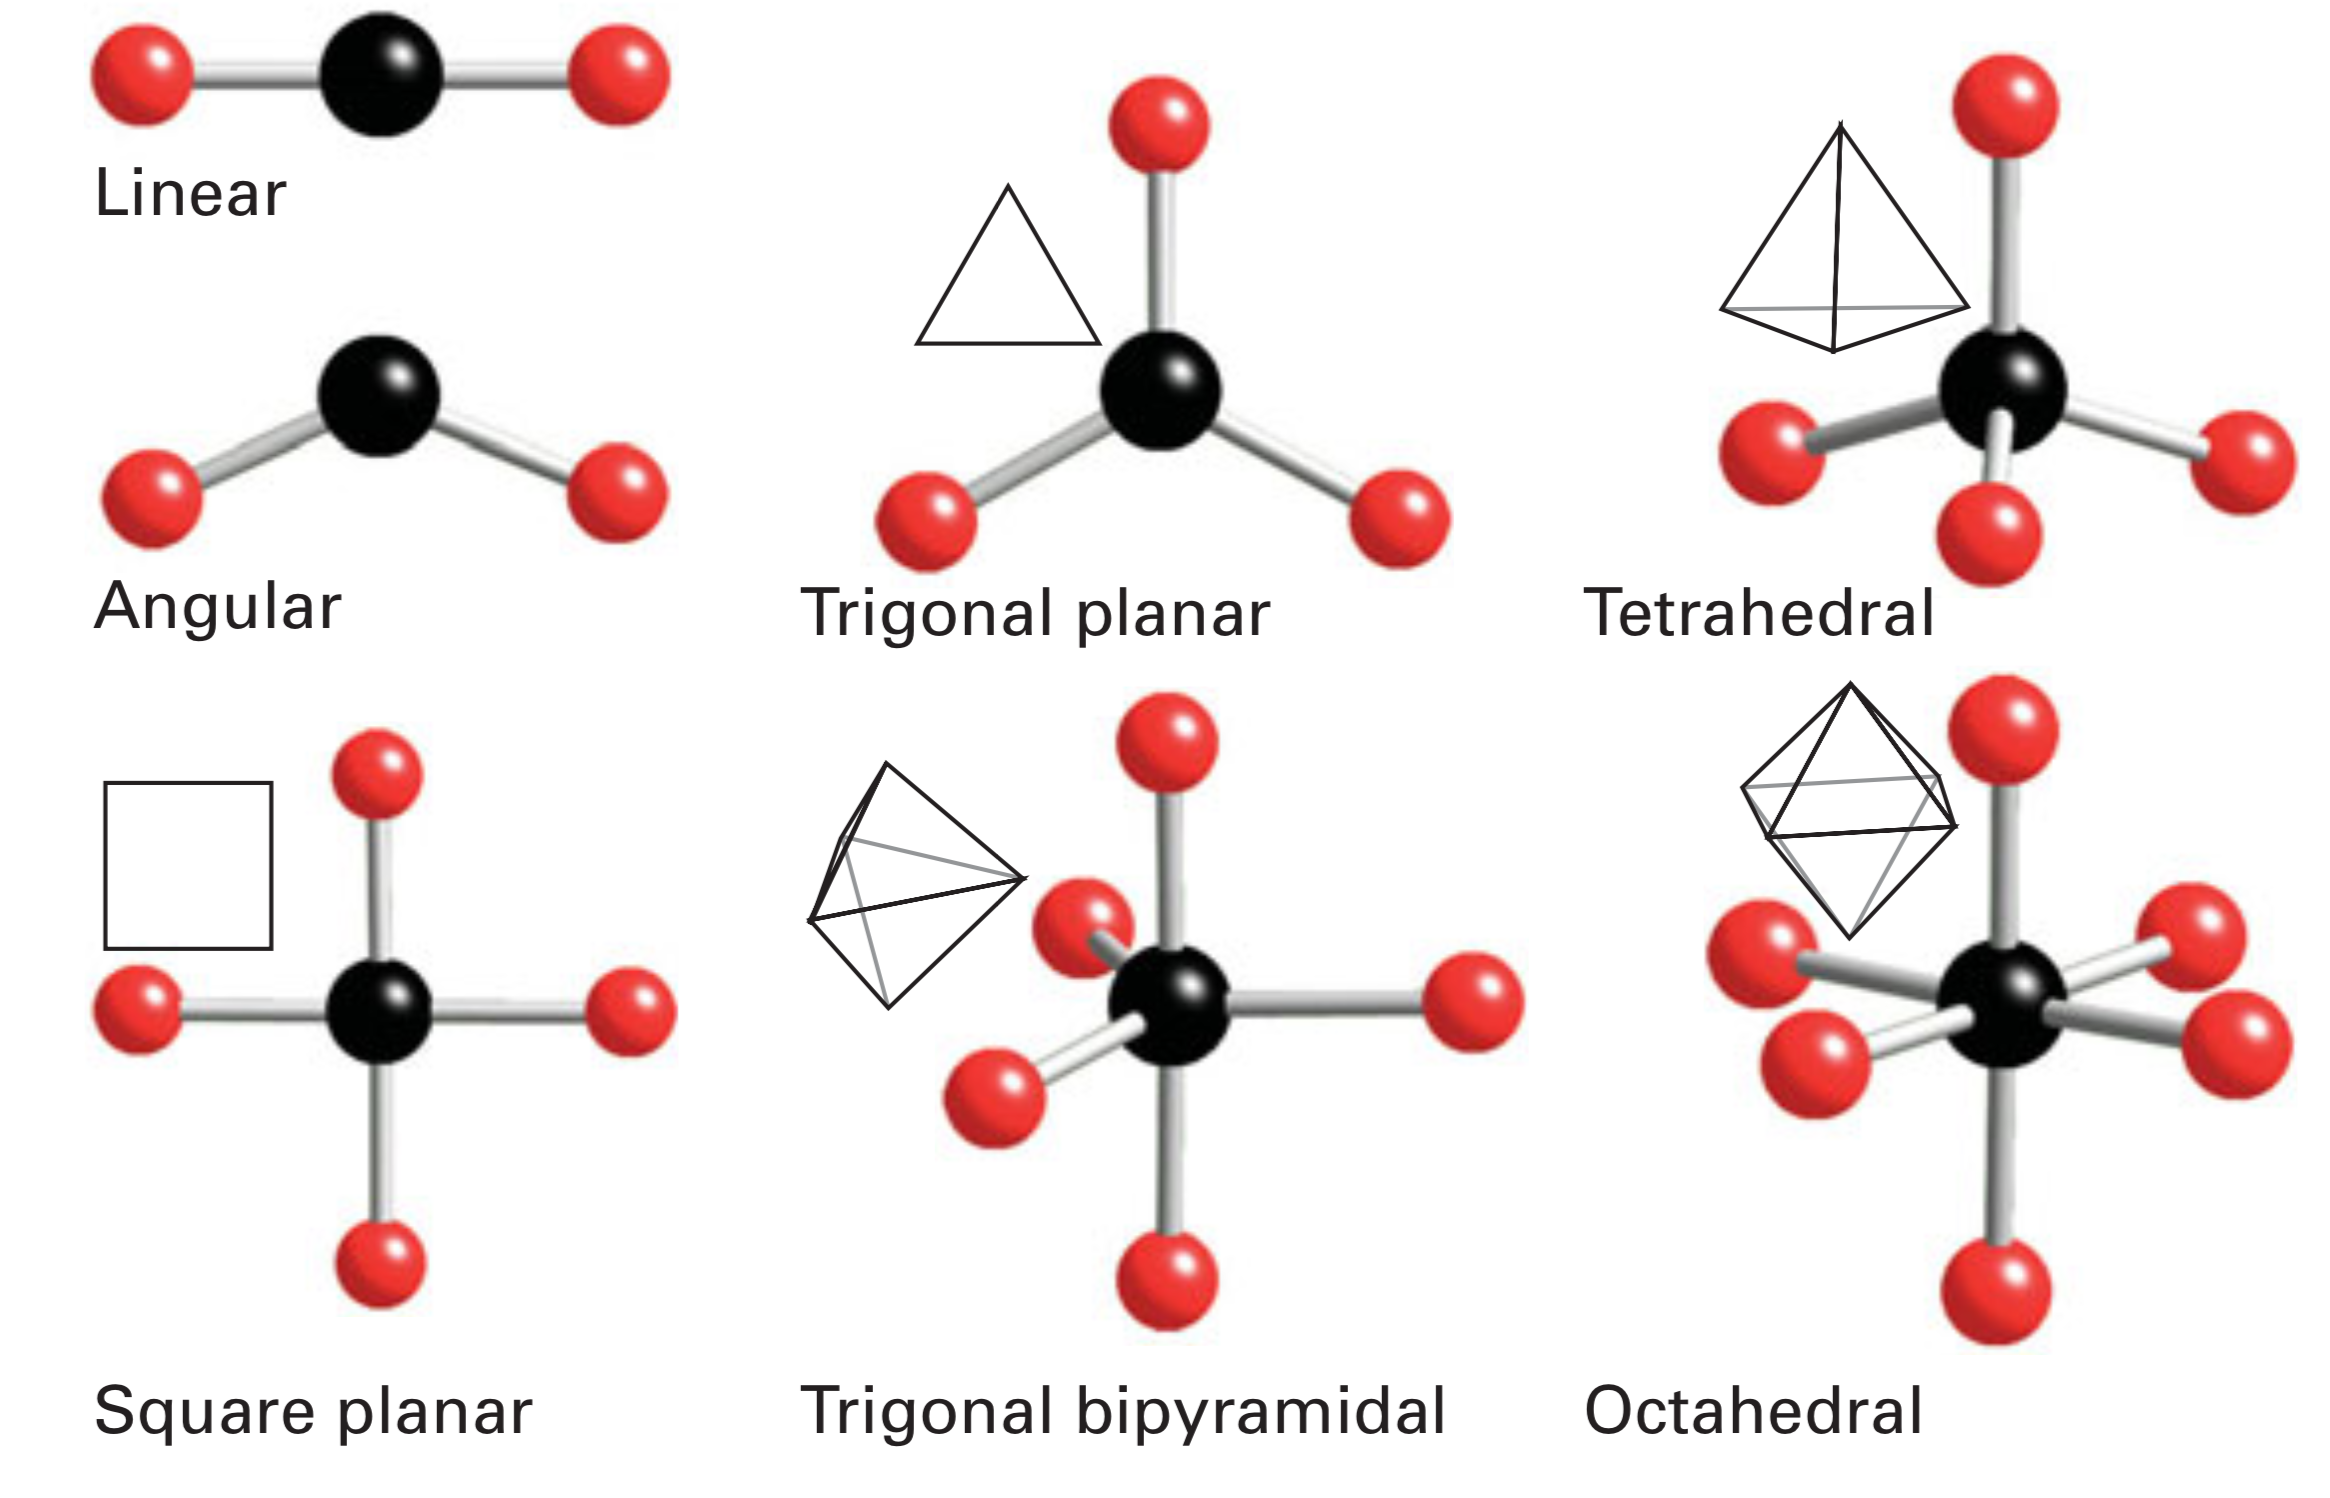
\includegraphics[width = 0.55\textwidth]{molecule_shapes.png}
        \caption{The geometric shapes used to describe symmetric, polyatomic molecules. In our examples, CO$_2$ is linear, H$_2$O is angular (or bent), CH$_4$ is octahedral, and SF$_6$ is octahedral. Figure taken from Atkins' \emph{Physical Chemistry} \citep{atkins2014physical}}
        \label{fig:shapes}
    \end{figure}

    Carbon dioxide is a linear molecule with the carbon atom in the middle of two oxygen atoms, water is a bent molecule, methane is tetragonal, and sulfur hexafluoride is octahedral. All four of these molecules' shapes can be visualized in Figure~\ref{fig:shapes}.

    Some atoms are more \textbf{electronegative} than others. That is, some atoms attract electrons more strongly than others. The net result of this leads to a partial negative charge (denoted $\delta^-$) near the atoms that are more electronegative and a partial positive charge (denoted $\delta^+$) located somewhere else on the molecule. When this occurs and there is an unequal sharing of electrons, we say that that the covalent bonds are \textbf{polar}. Now, when there are two opposite charges $Q$ separated by a distance $d$, then there is something that we call an electric \textbf{dipole moment}, $\mu$, whose magnitude is given by \( \mu = Q d. \) So when there are two different atoms bonded together, there will be a nonzero dipole moment. However, for the molecule \emph{as a whole}, there may not be any net dipole moment. For example, the double bond between carbon and oxygen in carbon dioxide is polar with the oxygen atom being more electronegative than the carbon. Thus, there is a dipole moment. However, since there is an identical dipole moment pointing in the \emph{opposite direction}, they cancel and thus, there is no overall dipole moment in carbon dioxide. In fact, of all the molecules we are going to discuss, only water has a non-zero dipole movement. Dipole moments will dictate the absorption of infrared light in Sec.~\ref{sec:sym_phys_prop} below \citep{atkins2014physical,harris1978symmetry,bishop1993group}

     % section bonding (end)

    \section*{\label{sec:sym_ops}Symmetry Operations and Elements} % (fold)

    Some objects are more symmetric than others. For example, a circle is more symmetric than a square. You are able to rotate a circle about its center by any angle and get a similar object. However, you are only able to rotate a square about its center by \SI{90}{\degree}, \SI{180}{\degree}, \SI{270}{\degree} and get back the same shape that you started with. Similarly, a sphere is more symmetric than a cube. An operation that transforms an object and leaves it looking the same is called a \textbf{symmetry operation.} The \textbf{symmetry element} about which a symmetry operation is performed which can be a line, point, or a plane. For example, a reflection is performed about a particular plane of an object. There are five symmetry operations that we will consider in this text:
    \begin{enumerate*}[(1)]
        \item identity, 
        \item reflections, 
        \item rotations, 
        \item improper rotations, and
        \item inversions.
    \end{enumerate*}
    We will treat and tackle each of these below.

        \subsection*{Identity} % (fold)
        \label{sub:identity}
        
        This is the simplest symmetry operation that every object has is the \textbf{identity} and is denoted by $E$. This operation tells you to do nothing to the object. The reason we include it is because some objects only have this symmetry and it is needed to satisfy certain mathematical requirements that we will not discuss here.

        % subsection identity (end)

        \subsection*{Rotations} % (fold)
        \label{sub:rotation}

        Another common symmetry operation that you may encounter is the \textbf{n-fold rotation} which we denoted by $C_n$; this means that we can rotate an object by $\SI{360}{\degree}/n$ and get back an equivalent object.\footnote{It's important to make the explicit distinction between \emph{equivalent} and \emph{identical}. An equivalent object looks like the same object that you started with. An identical object is the object that you started with. For example, rotating a triangle by \SI{120}{\degree} gives you an equivalent object whereas rotating it by \SI{360}{\degree} gives you the identical triangle.} It makes no difference whether you choose to rotate the object in a clockwise or counterclockwise direction, so long as you are consistent.In this text, we will choose the clockwise direction. 

        You can perform an $n$-fold rotation an arbitrary, integer number of times, say $m$ so long as $m$ is smaller than $n.$ We denote $m$ rotations about the $n$-fold rotation axis as $C^m_n$.  For example, if you rotate a square by \SI{180}{\degree} then you have just performed the $C^2_4$ operation which is also the same as a $C_2$ rotation. In other words \[ C_4 \cdot C_4 = C^2_4 = C_2\]. Furthermore, if you start with a square, rotate it by \SI{90}{\degree} and then rotate this equivalent object by another \SI{270}{\degree} you get the identical object that you started with. It's as if you hadn't rotated it at all! We call denote the operation that gives back the identity the \textbf{inverse.} More mathematically, we write \[C^3_4 \cdot C_4 = C^4_4 = E.\] In general, we can see that $C^{n-m}_n$ and $C^m_n$ are inverses of each other, i.e. $C^{n-m}_n \cdot C^m_n = C^{m}_n \cdot C^{n-m}_n = E.$ 

        Some simple examples would be a triangle has a 3-fold rotation axis, i.e. you can rotate the triangle about its center by $\SI{360}{\degree}/3 = \SI{120}{\degree}$, a square has a 4-fold rotation axis, a pentagon has a 5-fold rotation axis, etc. As we saw in our square example, some objects have multiple rotation axes. Consider a hexagon. You can rotate the hexagon by \SI{180}{\degree}, \SI{120}{\degree}, \SI{60}{\degree} corresponding to $C_2$, $C_3$, and $C_6$ rotations respectively. The highest value of $n$ (in this case 6) is called the \textbf{principal axis}. 

        \begin{exercise}
            Name the different $C_n$ in a cube. There should be three not including the identity operation. What is the principal axis and how many principal axes are there? (\emph{Hint:} Look at the corners and edges of the cube.)
        \end{exercise}

        % subsubsection rotation (end)

        \subsection*{Reflections} % (fold)
        \label{sub:reflection}

        The next symmetry operator, one that is likely familiar to you, is the \textbf{reflection} through a plane which is denoted by the Greek letter $\sigma.$ The mirror plane can either be parallel or perpendicular to the principal axis. If the mirror plane is parallel, we label the mirror plane $\sigma_v$ where the $v$ stands for ``vertical'' and if it is perpendicular we label it as $\sigma_h$ where $h$ stands for ``horizontal.''

        \begin{figure}[ht]
            \centering
            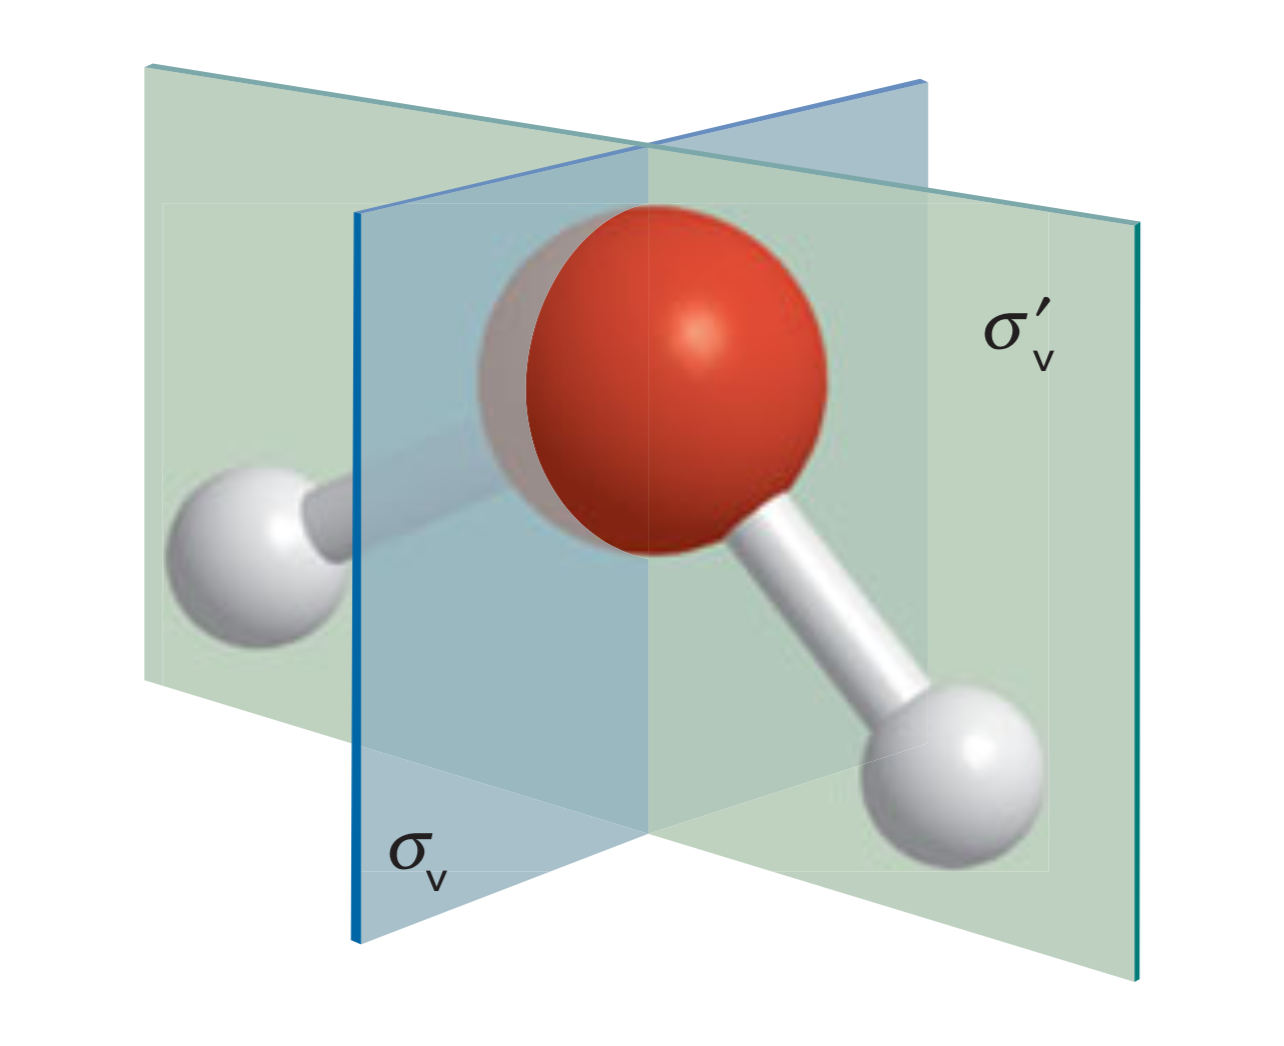
\includegraphics[width = 0.35\textwidth]{mirror_planes.png}
            \caption{An example of the two different mirror planes that correspond to the water molecule. Figure taken from Atkins' \emph{Physical Chemistry} \citep{atkins2014physical}}.
            \label{fig:mirros}
        \end{figure}

        Note that if you perform two reflections across the same plane in a row you get exactly what you started with, i.e. it's as if you performed the identity operation; more mathematically, we would describe it as such: $\sigma \cdot \sigma = \sigma^2 = E$. Therefore, we see that $\sigma$ is its own inverse.

        \begin{exercise}
            How many reflection planes does a square have? A rectangle?
        \end{exercise}
         % subsubsection reflection (end)

        \subsection*{Improper Rotations} % (fold)
        \label{sub:improp}

        This next symmetry operation is a little trickier to see and most of us don't have a good intuition for it like we might with proper rotations and reflections because it is a combination of the two. First you rotate the object by some amount and then reflect the object across a mirror plane that is perpendicular to the axis of rotation. See Figure~\ref{fig:improp_methane} for a visualization of this. We call this an \textbf{improper rotation} and denote it with the symbol $S_n$. The inverse of $S^m_n$, in general, is $S^{n-m}_n$ if $n$ is an even number and $S^{2n-m}_n$ if $n$ is an odd number. Can you see why we must make this distinction between $n$ being odd versus even?

        \begin{figure}[ht]
            \begin{center} 
            \begin{subfigure}[b]{0.35\textwidth}
                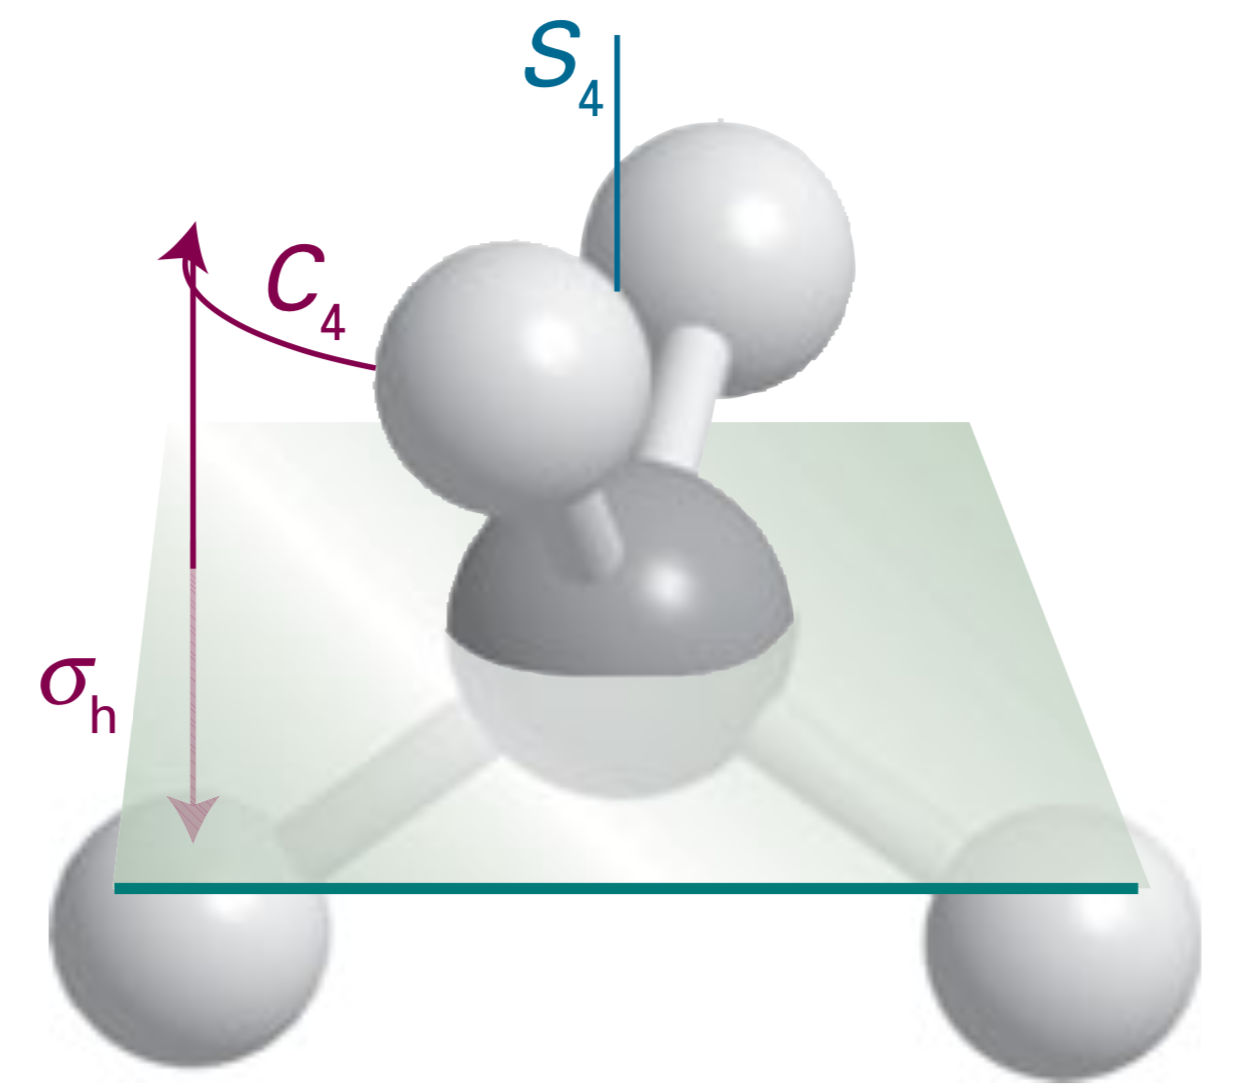
\includegraphics[width = \textwidth]{improper_methane.png}
                \caption{Methane}
                \label{fig:improp_methane}         
            \end{subfigure}
            ~
            \begin{subfigure}[b]{0.33\textwidth}
                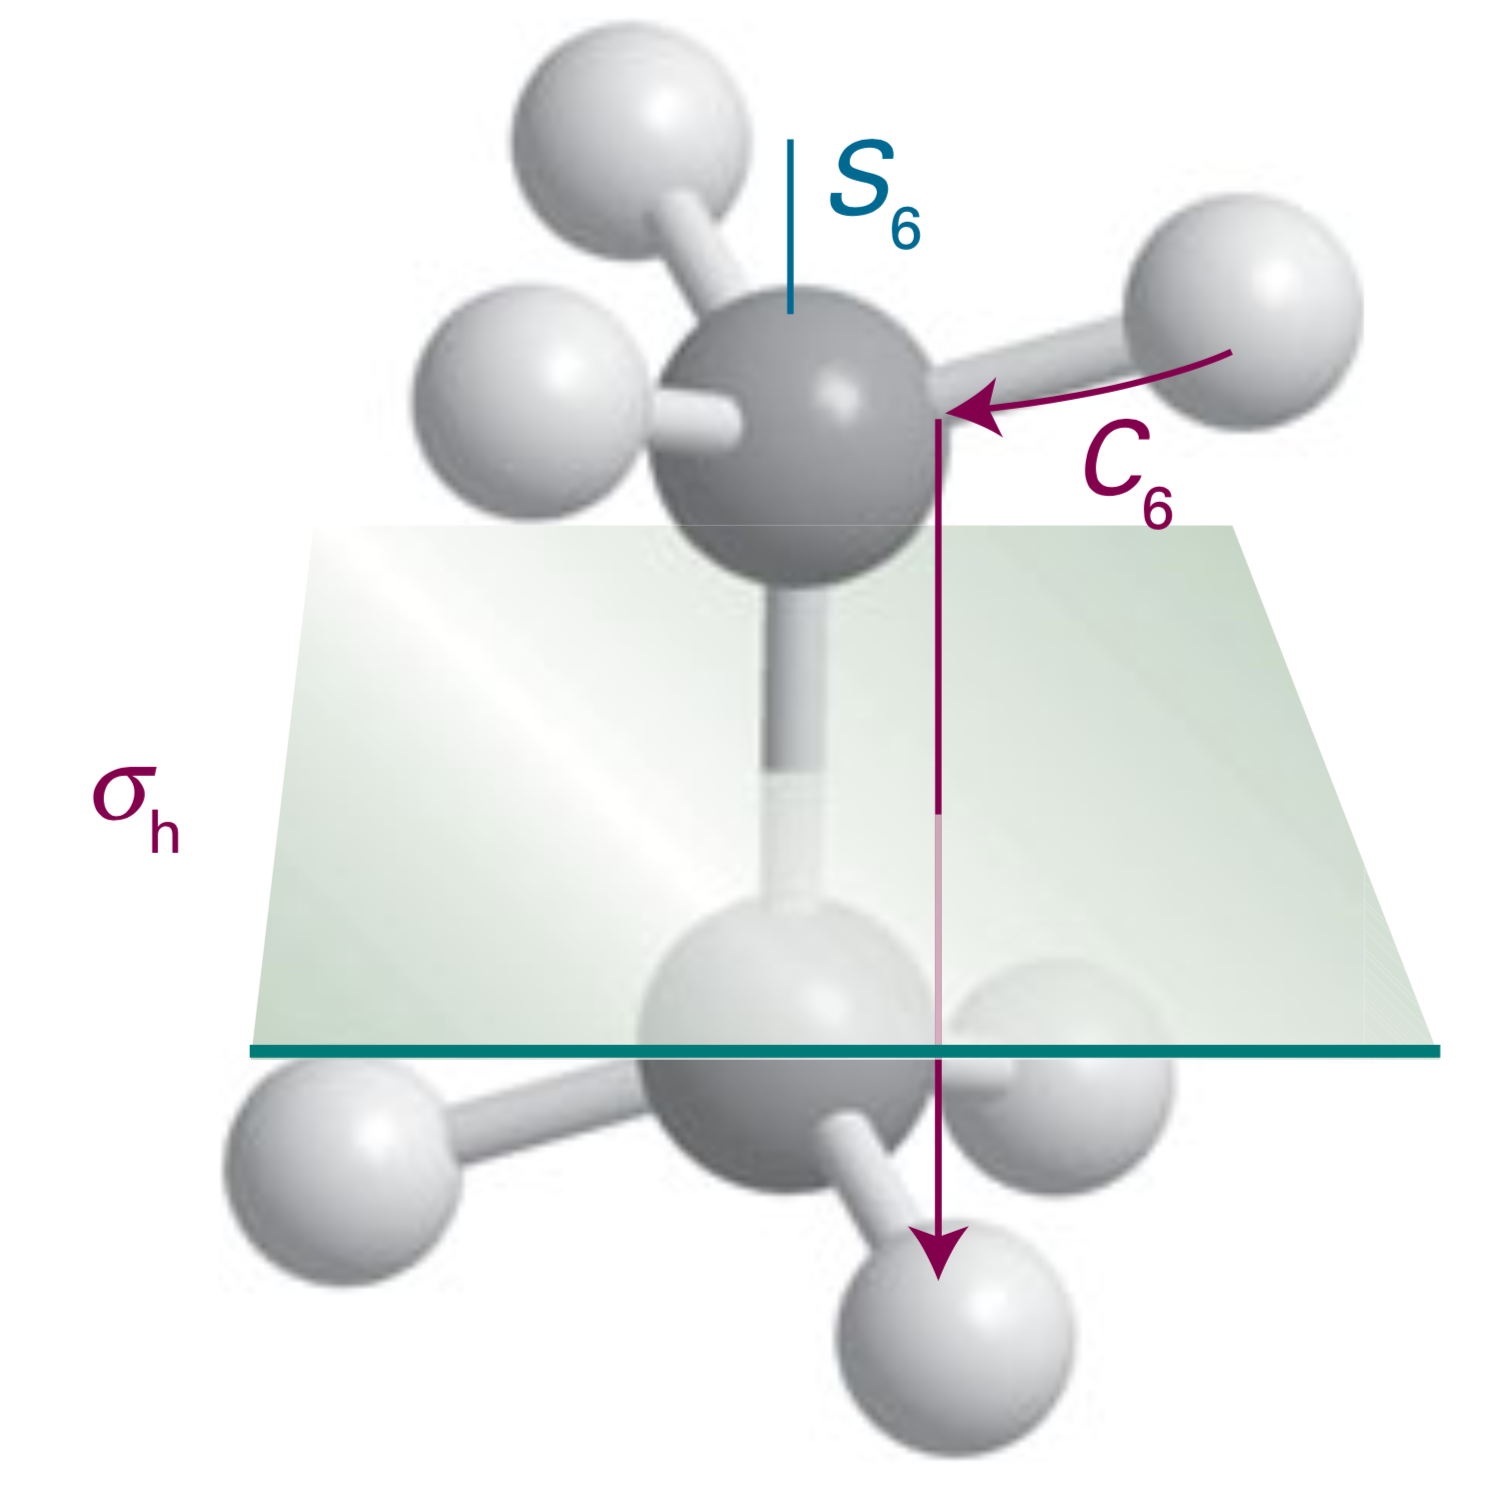
\includegraphics[width = \textwidth]{improp_ethane.png}
                \caption{Staggered Ethane}
                \label{fig:improp_ethane}         
            \end{subfigure}
            \caption{\textbf{(a)} A visualization of one of methane's three $S_4$ symmetry operations. First you rotate the molecule by \SI{90}{\degree} ($C_4$) and reflect it across the horizontal plane ($\sigma_h$). While neither the $C_4$ or $\sigma_h$ operation is a symmetry operation of methane by itself, by combining them together we see the molecule is indistinguishable (or equivalent) from what we started with. \textbf{(b)} Similarly for ethane only with at $S_6$ rather than $S_4$. Figure taken from Atkins' \emph{Physical Chemistry} \citep{atkins2014physical}}
            \label{fig:improper}
            \end{center}
        \end{figure}
        
        % subsubsection improper_rotation (end)


        \subsection*{Inversion} % (fold)
        \label{sub:inversion}
        The final symmetry operation we will go over is \textbf{inversion} which is represented as $i$ in symbolic form.\footnote{This is not to be confused with the same $i$ you may have encountered in a mathematics course previously where $i = \sqrt{-1}$ by definition.} We imagine passing each point in an object through its \textbf{center of symmetry} and placing it on the opposite side. If a point initially has the coordinates $(x,y,z)$ then after the inversion the coordinates will become $(-x,-y,-z).$ It turns out that this operation is equivalent to an $S_2$ operation (i.e. $i = S_2$), but inversion's importance warrants the distinction. An example of an object is the staggered ethane molecule shown in Figure~\ref{fig:improp_ethane}. Note that inversion is its own inverse.

    \begin{exercise}
       Find and sketch an objects that has inversion symmetry.
    \end{exercise}
        
        % subsubsection inversion (end)
    \begin{exercise}
     The Great Pyramid of Giza is one of the world's seven ancient wonders. Name and draw seven symmetry operations it has.
     \label{ex:giza}
    \end{exercise}

    \begin{exercise}
        Name all of the symmetry operations for
        \begin{enumerate*}[(a)]
            \item carbon dioxide,
            \item water,
            \item methane, and
            \item sulfur hexafluoride.
        \end{enumerate*}
    \end{exercise}

    % subsection symmetry_operations (end)    

    \section*{Physical Properties and Symmetry} % (fold)
    \label{sec:sym_phys_prop}

    Now at this point, you may be wondering why we went over this discussion of symmetry, much less in an environmental science textbook. The answer is that symmetry plays a fundamental role in how the natural world works around us.\footnote{
        The details are not important, but if you think of various conservation laws you may have heard of in various sciences courses (e.g. conservation of energy, conservation of linear and angular momentum, conservation of charge, etc.) all arise from various symmetries of systems that we are studying. This isn't important to this text, but it does show how interesting Nature is.
        } 
    So it should be no surprise that properties (both physical and chemical) arise from the symmetries of its structure. 
    
    Molecules can essentially do three things. They can translate across space. They can rotate. And lastly, they can vibrate.

    Now let us consider a single particle floating in free space by itself. There are only three ways for it to move, either in the $x$, $y$, and $z$-directions respectively. Because there are three ways for it to move, we say that there are three \emph{degrees of freedom.} Now when there are two particles moving together in free space, there are a total of six degrees of freedom. Three of the six include simple translation. That is, the molecule can move around. There are two ways it can rotate. This is a subtle point that only holds for diatomic molecules. In Figure~\ref{fig:diatom_dof}, we see that there is no way for a diatomic molecule to rotate about its $z$-axis, leaving one degree of freedom left for vibration. 

    \begin{figure}[ht]
         \centering
         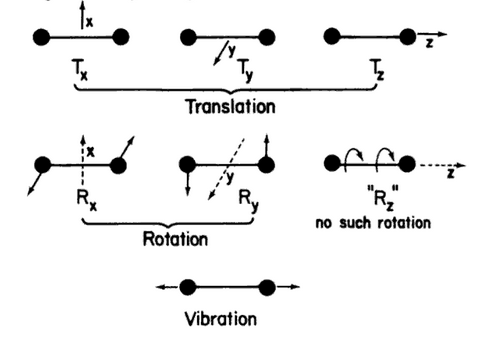
\includegraphics[width = 0.45\textwidth]{diatom_dof.png}
         \caption{The six degrees of freedom of a diatomic molecule. Notice that there are only two ways that it can rotate. The rotation about the $z$-axis does not change the location of the atoms, and thus, does not count (However, in any non-linear molecule, there will be a $R_z$ rotation). Because of this, there is a remaining degree of freedom: a vibrational one. Figure taken from Harris' \emph{Symmetry and Spectroscopy} \citep{harris1978symmetry}}.
         \label{fig:diatom_dof}
     \end{figure} 

    In principle, we can continue to just add more and more atoms to the molecules, making them bigger and bigger. With each atom, we get three more degrees of freedom. When the molecules are not linear, six of the degrees of freedom are contained within translation and rotation. The remaining degrees of freedom are turned into various vibrations of the molecule. To summarize, in a molecule with $N$ atoms, if the molecule is \emph{linear} there are $3N -5$ vibrational modes; if it is not linear, there are $3N-6$ vibrational modes.

    \begin{exercise}
        How many modes of vibration are there for 
        \begin{enumerate*}[(a)]
            \item carbon dioxide,
            \item water,
            \item methane, and
            \item sulfur hexafluoride?
        \end{enumerate*}   
        \label{ex:vib_numbers}
    \end{exercise}

    A logical next question would be, why do we care how many vibrational modes a molecule has? Quite simply, the answer is that when one of these vibrational modes is excited, the molecule \emph{absorbs} energy. Molecules can be thought of various atoms attached together with springs (the covalent bonds). When you have a mass on a spring, you can put energy into the system by displacing the mass by either compressing or stretching the spring. When you release the spring, the mass will vibrate back and forth. The same thing happens with molecules. The covalently bonded atoms act in the same way only with light exciting the bonds (springs), allowing the molecule to absorb energy and later radiate it back towards the earth contributing to the greenhouse effect.

    Now depending on the symmetry of the molecule, that is what symmetry operations each molecule has, determines how a molecule can vibrate. The different ways a molecule can vibrate are called \textbf{vibrational modes}. Here is the key concept to take away: a molecule will only absorb infrared radiation if the vibrational mode \emph{changes the overall dipole moment of the molecule.} \citep{harris1978symmetry,atkins2014physical,bishop1993group}. When a molecule absorbs IR-radiation, it is said to be \textbf{infrared active}. To further illustrate this, we will look at the case of water and carbon dioxide as seen in Figure~\ref{fig:vib_modes}. 

    \begin{figure}[hb]
     \begin{center}
        \begin{subfigure}[b]{0.6\textwidth}
            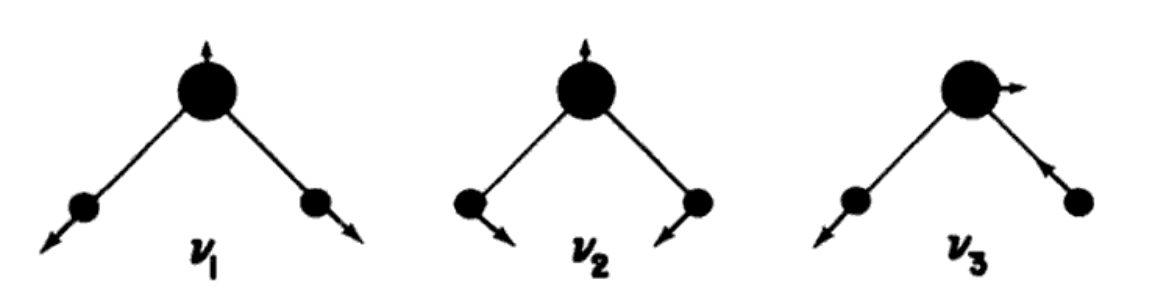
\includegraphics[width = \textwidth]{h2o_vibs.png}
            \caption{Vibrational Modes of H$_2$O. Figure taken from Harris' \emph{Symmetry and Spectroscopy} \citep{harris1978symmetry}}
            \label{fig:h2o_vibs}         
        \end{subfigure}
        \begin{subfigure}[b]{0.6\textwidth}
            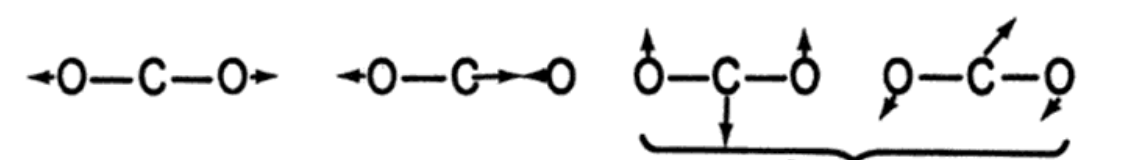
\includegraphics[width = \textwidth]{co2_vibs.png}
            \caption{Vibrational Modes of CO$_2$. Figure taken from Harris' \emph{Symmetry and Spectroscopy} \citep{harris1978symmetry}}
            \label{fig:co2_vibs}         
        \end{subfigure}
        \caption{Here are the vibrational modes of water and carbon dioxide. Every single way that either of these two molecules can vibrate is some combination of the modes given above. Only some of these are infrared active \citep{harris1978symmetry} N.B., the underbrace below the rightmost CO$_2$ vibrational modes are there to suggest that these are excited by the same energy, i.e. they are degenerate.}
        \label{fig:vib_modes}
     \end{center}
    \end{figure}    

    The dipole moment of water that is not vibrating, has a net dipole moment where the negative charge is centered near the oxygen atom and the positive charge is centered directly between each of the hydrogens.\footnote{
        Imagine drawing an arrow of length $d$ from the positive to the negative charge as a visualization of $\mu.$
        }. 
    If you go through each of the three vibrational modes of water given in Figure~\ref{fig:h2o_vibs}, then you will see that either the distance or direction of its this arrow, its dipole moment, will change. Consequently, each of the three ways that water can vibrate will absorb IR-radiation. However, if we look at carbon dioxide in Figure~\ref{fig:co2_vibs}, we see the left-most vibrational mode has zero net change in carbon dioxide's dipole moment as there is still an equal but opposite dipole moment pointing from the carbon atom to each oxygen; consequently, that vibrational mode is \textbf{infrared inactive.}

  
    Now we are finally understanding how important a molecule's symmetry actually is in determining its potency as a greenhouse gas. In the case of methane\footnote{Check out \texttt{http://www.chemtube3d.com/vibrationsCH4.htm} to visualize the vibrational modes of methane.} and sulfur hexafluoride,\footnote{Check out \texttt{http://www.chemtube3d.com/vibrationsSF6.htm} to visualize the vibrational modes of SF$_6$.} there are a relatively high number of atoms (5 and 7 respectively) leading to $3N - 6$ vibrational modes. If a molecule is highly symmetric, then essentially any vibration will change it's nonzero, net-dipole moment, leading to vibrations in the molecule that will absorb (and eventually re-emit) infrared radiation. This, coupled to with the lifetimes of these molecules in the atmosphere, make highly symmetric molecules much more potent greenhouse gases. As human-induced greenhouse gases (mostly carbon dioxide and methane) are the main contributers to climate change, it is important to understand how and why these gases have the relative potency that they do.

    \begin{exercise}
        Which of the following molecules are greenhouse gases: N$_2$, H$_2$, CF$_4$, and N$_2$O. Why?
        \label{ex:greenhouse_examples}
    \end{exercise}
    % section symmetry_and_physical_properties (end)



%%%%%%%%%%%%%%%%%%%
%% ANSWER KEY
%%%%%%%%%%%%%%%%%%%%%
\newpage
\section*{\label{app:answers}{\LARGE{Appendix B:}}\\Answers to Selected Exercises}
    \textbf{Solution~\ref{ex:kelvin}}: \begin{enumerate*}[(a)]
        \item \SI{273.15}{\kelvin}, 
        \item \SI{373.15}{\kelvin}.
    \end{enumerate*} \\
    \textbf{Solution~\ref{ex:humans}}: \begin{enumerate*}[(a)]
        \item \SI{734.51}{\watt}, 
        \item Assuming 2000 Cal/day: 32\% of food energy goes to body heat.
    \end{enumerate*}
    \\
    \textbf{Solution~\ref{ex:venus}}: \begin{enumerate*}[(a)]
        \item \SI{333.2}{\kelvin}, 
        \item \SI{230.8}{\kelvin}, and
        \item \SI{669.8}{\kelvin}.
    \end{enumerate*}   
    \\
    \textbf{Solution~\ref{ex:giza}}: $E,\, C_4,\, C_2,\, 4 \sigma_v.$ \\
    \textbf{Solution~\ref{ex:vib_numbers}}: 4, 3, 9, 15.  \\
    \textbf{Solution~\ref{ex:greenhouse_examples}}: CF$_4$, N$_2$O.